\begin{quote}
\textit{``Where are you?'' Hiro says.
\\
\\
``In Reality or the Metaverse?''
\\
\\
``Both.''}
\end{quote}
\hfill \textit{Snow Crash, Neal Stephenson}
\\
\\

%=========================================================================================================
%=========================================================================================================

\label{chapter-background}

% 'Position' section from experimental plan document

%\section{Introduction}

This chapter explores the ecosystem of alternate realities, studying models that have been introduced in attempts to corroborate the inherently subjective definitions and distinguishing features of different categories of alternate reality. A taxonomy of adopted definitions is used in order to introduce parallel reality in an unambiguous fashion as a new category of alternate reality. Moreover a new model for illustration of alternate reality experience is presented, through the combination of the reality-virtuality continuum of Milgram and Kishino with the three dimensions of virtual experience model of Waterworth and Waterworth, allowing for better explanation of the experiential aspect of the parallel reality concept and the introduction of an extended definition of the vacancy problem.





%The combination of real and virtual environments in this manner is not fully encapsulated by any previously defined alternate reality terminology, thus it was necessary to explore the ecosystem of alternate realities in order to correctly frame the introduction of a new category in relation to previously established models.

%The closest existing label is that of cross reality, but where cross reality sought to address the vacancy problem by means of sensor and actuator infrastructure, allowing actions in one environment to manifest into the other, the concept introduced by this thesis instead adopts the approach of direct visual engagement with both constituent environments.





%This research centres around the design, development and evaluation of a hardware and software platform which allows its user to observe and move around their Real World (RW) environment whilst wearing a wide field of view (FOV), stereoscopic 3D, Head Mounted Display (HMD) which allows them to alternatively view an immersive Virtual Reality (VR) environment from the equivalent vantage point. This is achieved by combining a head-tracked HMD, webcams, an indoor positioning system (IPS) and a 3D game engine, into a mobile \textit{cross reality} (XR) interface.

%One of the distinguishing features of XR is that, by linking real and virtual environments more closely, it mitigates the `vacancy problem': \textit{``the noticeable and profound absence of a person from one world, either real or virtual, while they are participating in the other''}, which arises \textit{``because people do not currently have the means to be in more than one place (reality) at a time''}~\cite{Lifton2007a}.

%Previous XR research approached the vacancy problem by integrating sensor/actuator networks into the environments, such that actions in one could manifest in the other, however direct visual engagement with the virtual environment was only possible from static interfaces at pre-determined locations within the real environment~\cite{Lifton2007a, Dublon2011}. The platform discussed in this document addresses this shortcoming by providing a mobile interface for visual engagement with both environments of a XR system, allowing the user to transition between viewing their real environment and a virtual environment at any time while maintaining the freedom to move around them, multiplexing visual stimuli from their real surroundings and from a parallel, virtual `mirror world'~\cite{Gelernter1993}.

%=========================================================================================================
%=========================================================================================================

\section{Defining Alternate Realities}

Alternate realities, explored in the context of this thesis as any situation in which the environmental stimuli received by a subject have been somehow modified or mediated (often by computer), have received substantial attention in recent decades. These themes have been explored for purposes as diverse as education~\cite{Warburton2009} and new forms of data visualisation~\cite{Coleman2009} to medical~\cite{TenEyck2011} and military training~\cite{Qiu2009} in addition to ever present entertainment applications~\cite{Scherrer2008}. Although terms such as \textit{virtual reality} and \textit{augmented reality} are now relatively common, both in the scientific literature and in the mainstream press, definitions of alternate reality terms such as these have often been used in vague and even conflicting manners, thanks in no small part to the fundamental nature of virtuality itself.

\begin{quote}
	\textit{``It is a characteristic feature of virtuality that it causes puzzlement regarding its relation to reality''}~\cite{Brey2014}
\end{quote}

The subjective and debatable nature of alternate reality definitions has led to several models that attempt to facilitate better understanding of the distinctions between different categories of alternate reality, most prominent among them the work of Milgram and Kishino in introducing the taxonomy of the reality-virtuality continuum, but also in the work of Steve Mann and Roy Want. Unsurprisingly these models do not always agree upon their definitions of certain categories, in some instances even contradicting each other. Thus in order to introduce parallel reality in an unambiguous fashion it is necessary to study these existing models and declare which interpretations and definitions this thesis adopts.

%=========================================================================================================

\subsection{Milgram and Kishino's Reality-Virtuality Continuum}
\label{milgram&kishino}
Milgram and Kishino addressed the issue of alternate reality definitions in detail and can be accredited with introducing the terms \textit{augmented virtuality} and \textit{mixed reality} to the literature, prompted by their identification of the need for more encompassing terms to supplement the existing definitions of augmented reality~\cite{Milgram1999}.

%However despite these thorough and well-reasoned definitions being published originally in 1994, much of the subsequent literature studied for this review has adopted conflicting, or at least confusing and misleading, definitions.

One of the overbearing concepts that they introduced is that whilst both purely real and purely virtual environments do exist they should not be considered discrete alternatives but rather poles lying at opposite ends of a linear scale that stretches from an entirely real environment at one extreme to an ontologically parallel but entirely virtual environment~\cite{Qvortrup2002} at the other: the \textit{Reality-Virtuality continuum} (figure \ref{reality_virtuality_extent_of_world_knowledge_continuum}, top). The location of an environment along this continuum coincides with its location along a parallel \textit{Extent of World Knowledge continuum} (figure \ref{reality_virtuality_extent_of_world_knowledge_continuum}, bottom), where `world knowledge' refers to the amount of quantitative information that is associated with the content being presented to the user, or in other words how much of the environment is being `modelled' by a computer system.

\begin{figure}[h]
\centering

\includegraphics[width=\textwidth]{virtuality_continuum_extent_of_world_knowledge_continuum.png}
\caption{Milgram and Kishino's reality-virtuality continuum (top) and extent of world knowledge continuum (bottom).}
\label{reality_virtuality_extent_of_world_knowledge_continuum}
\end{figure}

With a purely virtual environment, the entire viewport must necessarily be computer modelled in order to be rendered and as such there is complete quantitative information about and between all objects being presented. At the opposite end of the continuum with a completely real environment where none of the viewport is computer modelled there is no quantitative information associated with the content being displayed. At any point between the extremes the environment consists of a mixture of some modelled and some non-modelled content, with the computer associating quantitative information to, and between, the virtual objects, but not necessarily to the real objects or between the virtual and real objects.

Carrying the continuum concept further, Milgram and Kishino illustrated their understanding of augmented reality and also introduced two new related terms; augmented virtuality and mixed reality. Mixed reality describes any environment that is neither completely real nor completely virtual; that is, it encompasses all positions on the continuum between the extremes. Augmented reality is used to describe a real environment upon which virtual objects are overlain and augmented virtuality is used to describe a virtual environment upon which objects sampled from the real world (such as video feeds) are overlain. Both augmented reality and augmented virtuality are encompassed by mixed reality.

An obvious question raised from studying the reality-virtuality continuum is at what point toward the centre of the continuum an environment changes from being augmented reality into augmented virtuality or vice-versa. The answer to this question lies with consideration of what `background' environment is receiving the augmentations.

If one were to take a viewport depicting a purely real environment and incrementally add more and more virtual objects, the environment's classification might intuitively seem to progress rightward along the continuum. Eventually, with the majority of the real environment obscured by virtual objects one might posit that the resultant environment should have passed the centre point of the continuum and come to rest somewhere in its right half, gaining the classification of augmented virtuality. Likewise if one were to take a viewport depicting a purely virtual environment and incrementally introduce more sampled real objects to it, one might posit that it would eventually pass the centre point of the continuum and come to rest in the territory of augmented reality.

Anthony Steed's extension to Milgram and Kishino's reality-virtuality continuum concept clarifies the fallacy in this thinking by explicitly illustrating the concept of the `primary environment':

\begin{quote}
\textit{``While it is quite clear that the intention of plotting this axis was not to claim that it was actually a continuum between real and virtual, it is nevertheless clear that the main `environment' could be one of three things: a purely virtual environment, the local environment, or a remote real environment\footnote{Telepresence~\cite{Sheridan1992a}.}. One can think about what the background of the environment that the users see is...''}~\cite{Steed2014}
\end{quote}

Considering the first case of taking a viewport depicting a real environment and incrementally adding more virtual objects to it, the resultant environment is necessarily always augmented reality as the primary environment, that is the background upon which the augmentations are being placed, is real. Similarly in the second case the resultant environment is necessarily always augmented virtuality, as it is a virtual background environment that is the subject of the augmentations.

%=========================================================================================================

\subsection{Steve Mann's Venn Diagrams}
\label{stevemannvenn}
Steve Mann, the \textit{``father of wearable computing''}\footnote{\url{http://www.theguardian.com/technology/2012/apr/05/google-project-glass-digital-goggles}} and one of a group of researchers at MIT that became known as `cyborgs' for their body-worn computers and always-on Internet connections~\cite{Turkle2011}, presented a Venn diagram to illustrate the relationships between the different categories of alternate realities, when reviewing the problems that arose with existing taxonomies in  discussion about reality-modifying devices.

Mann clarifies the use of the term `mediated reality' as \textit{``\ldots\ a general framework for artificial modification of human perception by way of devices for augmenting, deliberately diminishing, and more generally, for otherwise altering sensory input''}~\cite{Mann2002a}. Under this definition mediated reality encompasses all of mixed reality, but also the group of \textit{modulated reality} which covers devices such as eyeglasses that use lenses/mirrors to invert the wearer's view, but do not apply computer mediation or modification nor necessarily add or remove any content.

%Alone Together p 151

In this thesis, where we are concerned with alternate realities as those that are created or modified through means of computers or other apparatus (Mann's `devices'), one might want to consider the terms mediated reality and alternate reality to be one and the same. However in the larger consideration of virtual worlds as quoted in section \ref{intro-parallel-reality}, one might wish to reserve mediated reality specifically for the sub set of experiences that rely upon the application of `devices', whilst the super set of all alternate realities would contain, in addition, those experiences of simple imagination, storytelling and psychoactive agents.

Mann's Venn diagram (reproduced in figure \ref{Mann_venn_original.png} from the original in~\cite{Mann2002a}) situates augmented reality as a subset of mixed reality, in agreement with Milgram and Kishino. However it situates virtual reality as a subset of augmented reality, and in turn mixed reality, which does not agree with Milgram and Kishino. One interpretation of this decision is that Mann considers that virtual reality can exist as an extreme case of augmented reality where nothing but augmentations are present. However the position adopted by this thesis and illustrated in figure \ref{Mann_venn_mod_1.png} which presents a modified version of Mann's Venn diagram adopts the position of the reality-virtuality continuum more strictly. Although Mann and Milgram and Kishino seem to agree that virtual reality is necessarily mediated, this thesis adopts the position from Milgram and Kishino that it is not necessarily always presented as part of an augmented or mixed reality as Mann's diagram would seem to present.

%Mann himself states that \textit{``mixed reality exists in many forms along a continuum from augmented reality \ldots\ to more recent efforts at augmented virtuality''}, which is arguably contrary to his diagram's representation of virtual reality as a subset of augmented reality and in turn of mixed reality.

The modified diagram also features augmented virtuality in Milgram and Kishino's definition, mentioned by Mann in his prose but not included in his original diagram. An overlap is introduced here for those modulated reality environments that are also classified as mixed reality, as it is perplexing to think of a mixed reality environment that is neither augmented reality nor augmented virtuality, at least when considering a wholly real environment and a wholly virtual environment as the logically possible extremes, as in Steed's primary environments extension to the reality-virtuality continuum concept.

\TwoFig{Mann_venn_original.png} {Mann's Venn diagram of alternate realities, reproduced from~\cite{Mann2002a}.} {Mann_venn_original.png}
       {Mann_venn_mod_1.png} {Mann's Venn diagram of alternate realities.} {Mann_venn_mod_1.png}

\begin{figure}[h]
\centering
  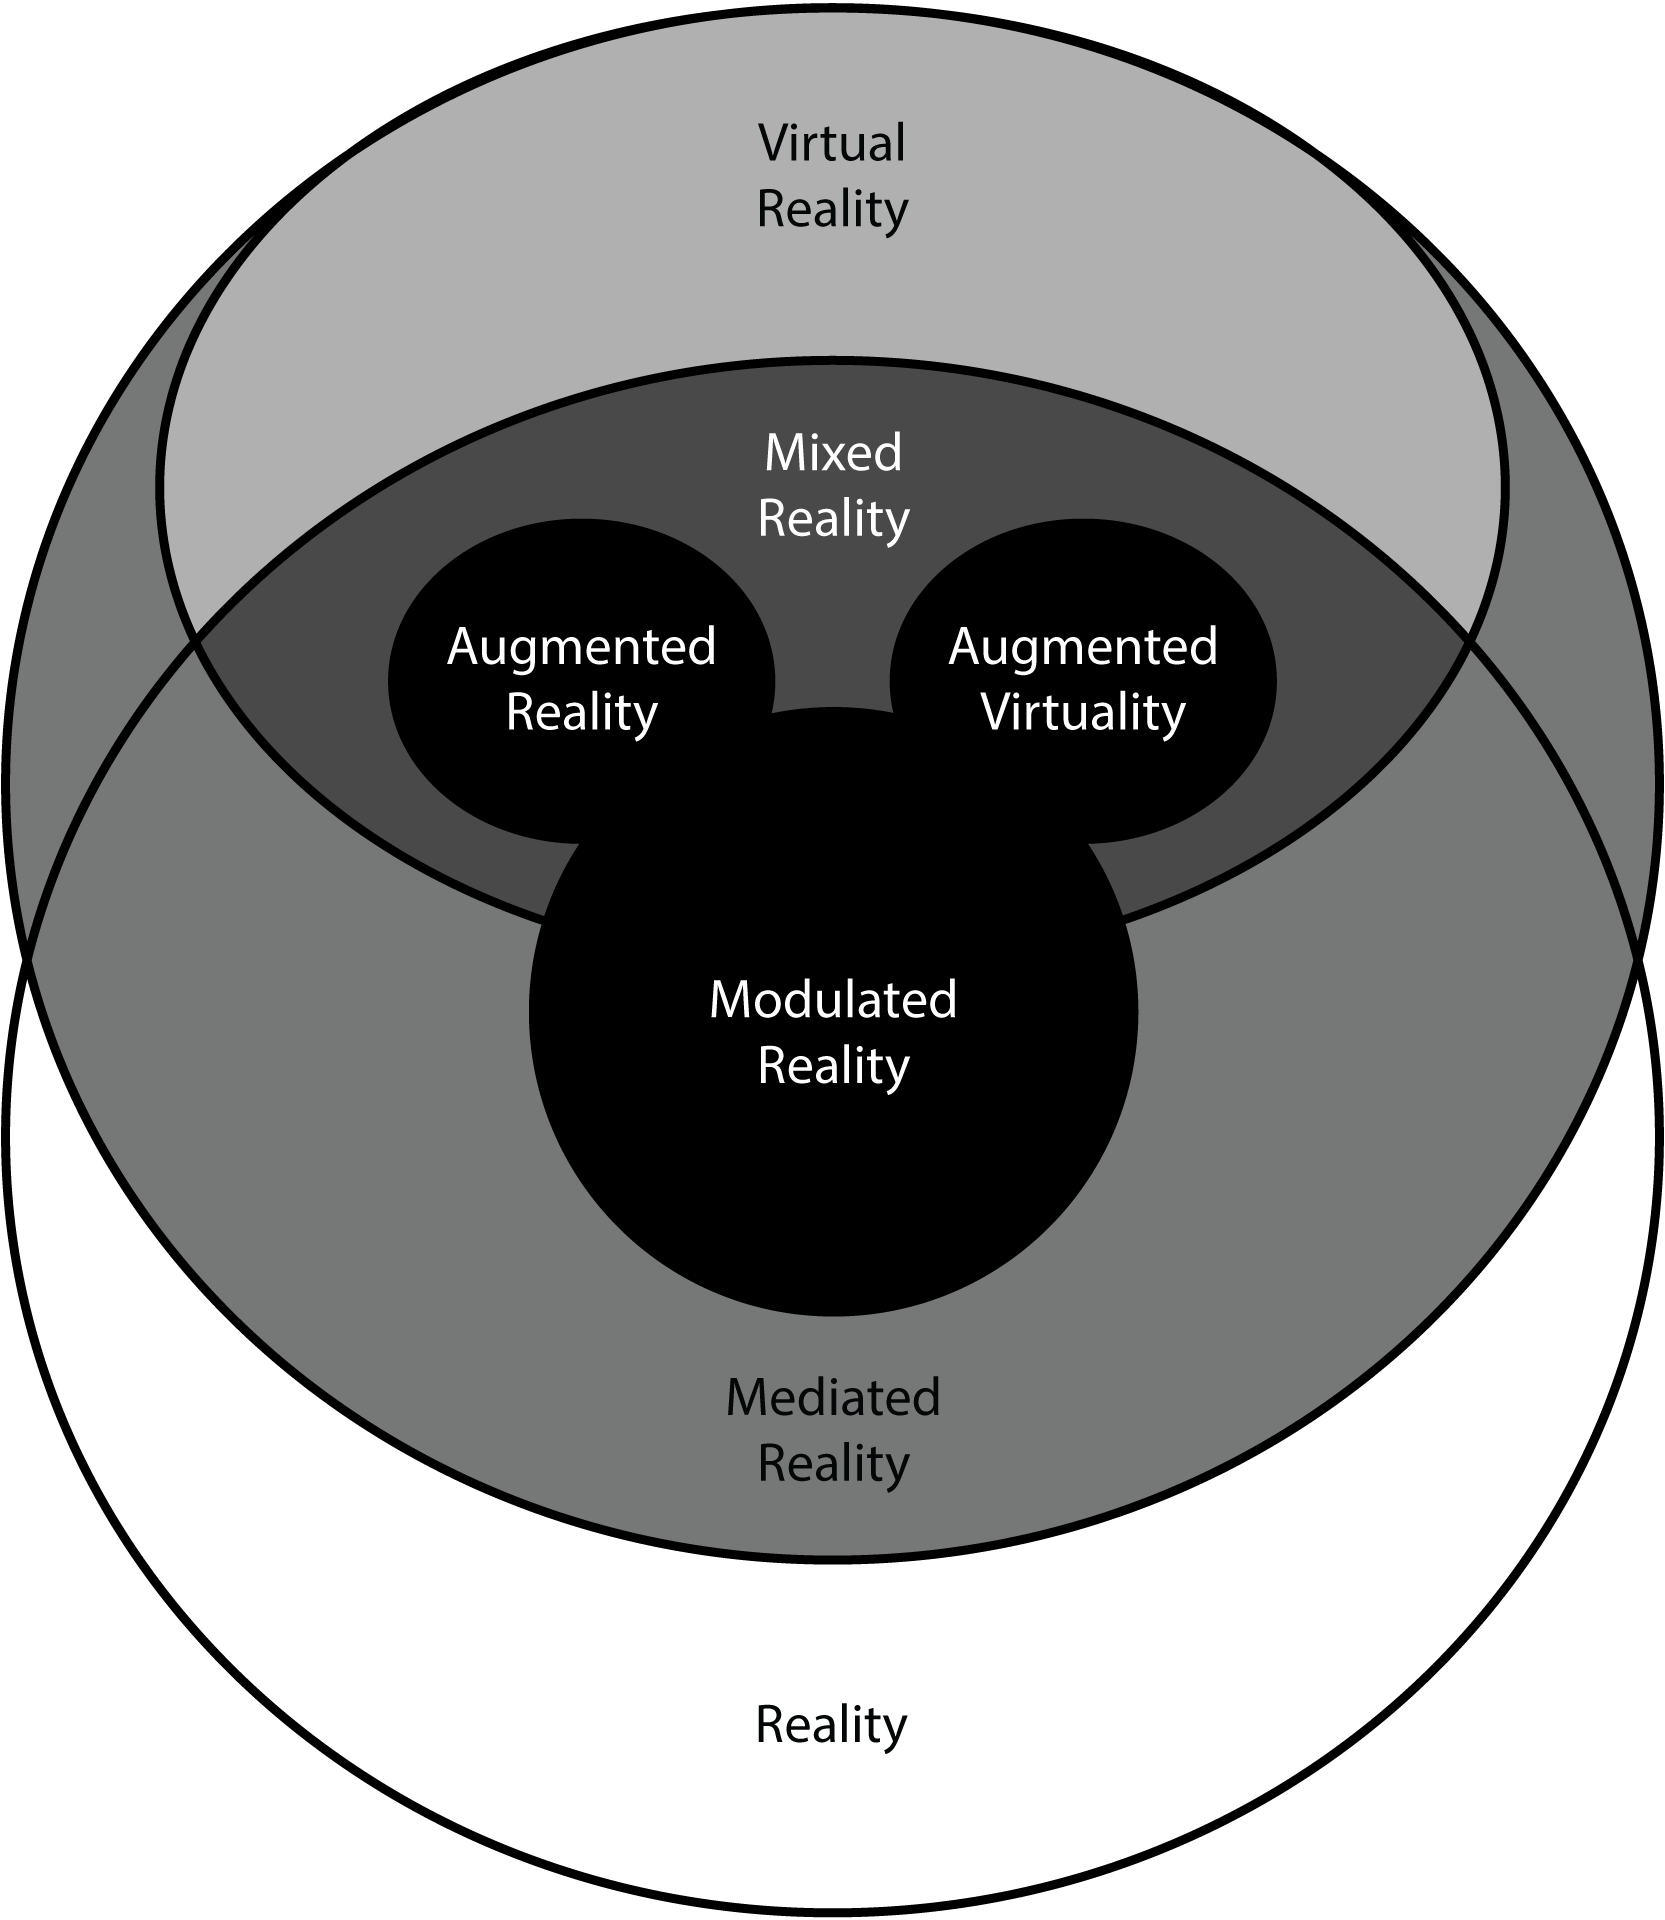
\includegraphics[width=0.5\linewidth]{Mann_venn_mod_3.png}
  \caption{Mann's Venn diagram of alternate realities after further modification.}
  \label{Mann_venn_mod_3.png}
\end{figure}

Visualising the position of Steed's primary environments, reality and virtual reality, using the same Venn diagram approach requires more drastic alteration, but is diagnostic in further corroborating the relationships between the terms covered in Mann's literature with others from the wider literature. The further modified Venn diagram (figure \ref{Mann_venn_mod_3.png}) shows that:
\begin{itemize}
	\item Mixed reality is the intersection of reality and virtual reality.
	\item Mediated reality can be comprised from purely real or purely virtual content.
	\item All virtual reality is necessarily mediated.
	\item Modulated reality can comprise only mediated real, or both real and virtual aspects in a mixed reality.
	\item Augmented reality and augmented virtuality can feature in modulated reality systems.
\end{itemize}

This final iteration of the Venn diagram still contains ambiguity, however it is more diagnostic for categorising the majority of alternate reality terms than the previous two diagrams, whilst also avoiding over-complication. There are two ambiguities to recognise. First, this diagram maintains from Mann's original diagram those positions in which a system can exist that is both mixed and modulated, but which is neither augmented reality nor augmented virtuality. Second, the diagram does not accommodate a purely virtual environment that is then modulated; whether such a system would ever be created is debatable, as any modulation that could be performed by modulators external to the virtual environment implementation could almost certainly be better performed by that virtual environment implementation itself.

%=========================================================================================================
\subsection{Roy Want's Virtuality Matrix}
\label{roy-wants-virtuality-matrix}
Another method of illustrating the relationships between different categories of alternate realities was put forward by Roy Want in his introductory article for a 2009 issue of IEEE Pervasive Computing~\cite{Want2009} dedicated to the cross reality paradigm (discussed in section \ref{sec_crossreality}). He presents a 2x2 matrix that categorises terms according to whether the experience and overlay data are real or virtual. As with Mann's Venn diagram some of the resulting definitions produced by Want's matrix, reproduced in figure \ref{Want_virtuality_matrix_original.png} from the original in~\cite{Want2009}, differ from those of the reality-virtuality continuum and the wider literature; indeed some of the criteria would seem to conflict with those adopted by other authors within the same issue of Pervasive. While the subjective nature of virtual experience admonishes labelling either as more `correct' than the other, this nonetheless serves as a prime example of the importance of clearly stating which definitions will be adopted by this thesis before introducing the parallel reality concept, in order to avoid ambiguity.

\TwoFig{Want_virtuality_matrix_original.png} {Want's virtuality matrix, reproduced from~\cite{Want2009}.} {Want_virtuality_matrix_original.png}
       {Want_virtuality_matrix_modified.png} {Want's virtuality matrix after modification.} {Want_virtuality_matrix_modified.png}

Figure \ref{Want_virtuality_matrix_modified.png} presents a modified version of Want's matrix that meshes more closely with the framework laid out by Milgram and Kishino and the definitions ultimately adopted by this thesis for framing parallel reality within. Where the original matrix positions cross reality in the upper left quadrant, the modified matrix instead positions augmented virtuality. The congruence of `experience virtual' and `overlay data real' would seem to hint toward a position within the right half of the reality-virtuality continuum and a single partially modelled environment, rather than eliciting ideas of the two discrete environments, one real and the other virtual, that the cross reality and parallel reality concepts capture.

The original matrix also features the term embodied virtuality, in the upper right quadrant at the congruence of `experience real world' and `overlay data real'. Want explains that embodied virtuality is used here as an alternative term for \textit{ubiquitous computing} which he considers to be \textit{``essentially the opposite of VR''} and describes the integration and dissemination of computational infrastructure into our real surrounds~\cite{York2004}. While the reality-virtuality continuum concept and the position taken by this thesis posit that the opposite of VR is simply reality, as shown in the modified matrix in figure \ref{Want_virtuality_matrix_modified.png}, an equally valid alternative position (and perhaps that held by Want) is that tangible interfaces can be employed to embody aspects of a virtual world that have no physical counterpart in the real world, to present physical abstractions of real world concepts or virtual world information, leading to the congruence of real overlay data and real experience as embodied virtuality.

%The modified matrix adopts the position that the opposite of virtual reality is simply reality and that ubiquitous computing does not constitute a category of alternate reality but rather a model of human-computer interaction (that can be implemented in either reality or augmented reality, depending upon how the ubiquitous computing infrastructure presents information to the user). A ubiquitous computing system is necessarily a real environment, as by definition it is the integration and dissemination of computational infrastructure into our real surrounds~\cite{York2004}. However whether this real environment is augmented by virtual objects is not restricted by the concept.

Finally on a more stylistic level, the modified matrix removes the central mixed reality section from the original matrix as its position could be misleading. Taking the boundaries between the sections literally, the reader could be led to believe that a purely virtual reality environment is also to be considered mixed reality, which is not a position proffered by Want nor by the wider literature. If one wished to picture the position of mixed reality upon the modified matrix, one would do better to picture it covering the area enclosed by the union of the augmented virtuality and augmented reality regions.

%=========================================================================================================

\section{Adopted Alternate Reality Definitions}
\label{summaryofalternaterealitydefinitions}

Table \ref{adopted-alternate-reality-definitions} presents the basic categories of alternate reality and their definitions as a product of the survey and update of the frameworks explored thus far. This table does not claim to present an exhaustive list of \textit{all} categories of alternate reality; rather, it presents the fundamental set of common categories that are required to move forward with the framing of parallel reality in a well grounded fashion. Terms such as HyperReality~\cite{Terashima2001} (capitalization important, to differentiate from the postmodern term `hyperreality'~\cite{Baudrillard1994}) are intentionally excluded due to their limited applications and exposure in the literature.

%HyperReality (HR) is the term given to a hypothetical communications infrastructure that allows the seamless commingling of reality and virtual reality, human intelligence and artificial intelligence. In terms of the previously explored alternate reality terms, a HR system is most accurately described as facilitating the creation of mixed reality environments that bring virtual reality content into real world locations $-$ \textit{``It seeks to make virtual reality something that is experienced as part of physical reality, so that virtual and real phenomena appear to interact with each other: HR is VR as well as, not instead of, PR''}~\cite{Terashima2001}.

%HR is an abstract, high level term that refers to a category of mixed reality environments that combine VR content with views of the real world in a manner that arguably falls under the moniker of augmented reality, however HR places emphasis on the integration of the virtual reality content into the real world in a seamless manner, such that HR enables hyperreality (this latter non-capitalised term referring to the postmodern usage of the word wherein an observer is unable to distinguish reality from a simulation of reality~\cite{Baudrillard1994}).

%=========================================================================================================

\newpage

\begin{center}
\begin{longtable}{ l p{10cm} }

\toprule

\textbf{Term} & \textbf{Definition} \\

\midrule

%=========================================================================================================
		
Reality & An environment that is entirely unmodelled, with the viewport containing no virtual objects and with no computer-based quantitative information associated with any of the (necessarily real) objects. One of the fundamental primary environments, occupying an endpoint of the reality-virtuality continuum. \\
		
\midrule
		
%=========================================================================================================

Alternate Reality & Any environment in which the environmental stimuli received by a subject have been somehow altered or changed. That is, alternate reality is a term that encompasses everything that isn't simple `reality'. \\

\midrule
		
%=========================================================================================================

Mediated Reality & \textit{``A general framework for artificial modification of human perception by way of devices for augmenting, deliberately diminishing, and more generally, for otherwise altering sensory input''}~\cite{Mann2002a}. Encompasses all of mixed reality and modulated reality. \\

\midrule

%=========================================================================================================

Modulated Reality & Platforms that aim to modify the user's view, by multiplicative, diminishing, rotational, etc. techniques, where the user's view can be wholly real, or a mix of real and virtual content, not necessarily adding or removing anything. \\

\midrule

%=========================================================================================================

%Telepresence & The ability for a user to experience a sense of presence at a real location remote to themselves~\cite{Sheridan1992a}. \\

%\midrule

%=========================================================================================================

Mixed Reality (MR) & The broad range of environments that arise from the merging of real and virtual environments to some extent, such that the result is neither entirely real nor entirely virtual, with real and virtual objects co-existing. Both augmented reality and augmented virtuality are included under the broader classification of mixed reality. \\

\hline
		
%=========================================================================================================

Virtual Reality (VR) & The polar opposite of reality, an environment that consists solely of virtual objects, with computer-based quantitative information associated with and between all of them, creating a completely synthetic world entirely discrete and separate from the real world; a new world that exists solely within the data structures of a computer~\cite{Milgram1999, Want2009}. One of the fundamental primary environments, occupying an endpoint of the reality-virtuality continuum. \\

& While traditional definitions of virtual reality require the environment to be completely immersive, such that when involved with the environment the user is completely unaware of the real environment that surrounds them (such as by using HMD and body tracking techniques to remove logical anchors to the real world\footnote{\url{http://www.techcastglobal.com/documents/10193/34869/++Aaron/aade1a72-900b-4261-9214-061fba89053d}}) one can also adopt less drastic criteria and classify the virtual environments presented by video games viewed via traditional computer monitors as rudimentary implementations of virtual reality - \textit{``a virtual reality accessed through standard personal computers is arguably very much in evidence in computer games''}~\cite{Green2014}. \\
		
\midrule

%=========================================================================================================

%Distributed Virtual Reality (DVR) & Multi-user VR where telecommunications are employed to allow multiple (geographically distributed) users to occupy the same VR environment, allowing cooperation~\cite{Terashima2001}. \\

%\midrule
		
%=========================================================================================================

Augmented Reality (AR) & A mixed reality environment that features a real environment as its primary environment and onto which virtual objects are added or overlain. A common approach for achieving this addition/overlay is superimposing virtual objects over a direct or indirect view of the real environment using HMD \&/or cameras~\cite{Krevelen2010}, more recently making use of smartphones with their built in cameras and orientation sensing capabilities. \\

	%A commercial example of \textit{augmented reality} is the Layar browser for mobile phones, which overlays various forms of data onto the view captured by a phone's camera after determining its location and orientation using GPS, accelerometer and magnetometer readings~\cite{eishita:layar}

%~\cite{Milgram1999}

\midrule

%=========================================================================================================

Diminished Reality & Where augmented reality is concerned with adding virtual objects to a view of the real world, diminished reality is concerned with the removal of objects from a view of the real world~\cite{Mann2002}. Simple applications include the removal of real world advertisements, such as billboards. More involved applications might combine diminished reality with augmented reality to, for example, present a faithful representation of a historical scene upon a real world environment, by not just adding historical artefacts via augmented reality but also removing historically inaccurate latter development via diminished reality. \\

\midrule

%=========================================================================================================

Augmented Virtuality (AV) & A mixed reality environment that features a virtual environment as its primary environment and onto which sampled real objects are overlain, perhaps through the use of cameras~\cite{caballero:behand}. \\

%A simple commercial example of augmented virtuality is the EyeToy accessory and associated software for Sony's Playstation 2 games console (and later the Playstation Eye for the Playstation 3), a digital camera that captures images of players and their surroundings and integrates them into the gaming experience presented on the screen.

\bottomrule
\caption{Summary of alternate reality definitions.}
\label{adopted-alternate-reality-definitions}
\end{longtable}
\end{center}

%=========================================================================================================

%\section{Introducing a New Alternate Reality}



%=========================================================================================================

\section{Cross Reality}
\label{sec_crossreality}

\newcommand{\SLfootnote}{\footnote{Second Life.}}

In order to introduce parallel reality as a new category of alternate reality, it is necessary to properly introduce one additional category of alternate reality to the ecosystem of alternate realities explored by the preceding sections: that of \textit{cross reality}. This is a more recent addition to the field of alternate realities, with its roots in the mid to late 2000s, than the more familiar terms covered in previous sections. However as one of its fundamental features is shared with parallel reality its inclusion in this discussion is required.

Cross reality (XR~\cite{kim:practical}) is a mixed reality situation that arises from the fusion of real-world sensor/actuator infrastructure with a complete virtual environment, facilitating synchronous bidirectional exchange of media and control information between real and virtual environments. Cross reality systems feature two environments, one real and the other virtual, both complete unto themselves~\cite{lifton:merging} but enriched by their ability to mutually reflect, influence and merge into one another thanks to bidirectional information flow between them~\cite{kim:practical}. Sensors collect and tunnel dense real-world data into virtual environments where they are interpreted and displayed to dispersed users, whilst interaction of virtual participants simultaneously incarnates into the real world through a plenitude of diverse displays and actuators~\cite{Paradiso2009}, such that actions within the virtual environment can have `extravirtual effects'~\cite{Soraker2010} upon the real environment and vice-versa.

The principle features that distinguish cross reality from the other alternate realities covered so far are:
\begin{enumerate}
	\item A shift from single- to bi-directional information flow between real and virtual environments~\cite{kim:practical}.
	\item That both the real and virtual environments are complete unto themselves (but are enriched by their ability to mutually reflect, influence and merge into one another)~\cite{lifton:merging}.
\end{enumerate}

As an alternate reality paradigm cross reality has its roots in work undertaken by the IBM Virtual Universe Community\footnote{\url{http://eightbar.co.uk/2006/04/22/lessons-from-second-life/}}\footnote{\url{http://eightbar.co.uk/2006/04/09/second-life-outside-in/}}\footnote{\url{http://eightbar.co.uk/2006/04/04/well-it-got-my-attention-second-life/}}, described in personal correspondence with Ian Hughes, a key figure in IBM's forays into Second Life:

\begin{quote}
\textit{``The control mechanisms worked two ways generally. There was a physical lab that had devices that were controlled by a pub/sub mechanism \ldots\ Those devices subscribed to various messages. So initially web pages controlled them \ldots\ Equally the objects generated messages when they were physically switched on and off. As SL\SLfootnote{} had an RPC interface it was possible \ldots\ to subscribe to the same messages and send requests into SL to change states of objects \ldots\ So there were lights, blinds, proximity detectors and even the tilt sensors on the laptops that were instrumented with these messages.''}
\end{quote}

It was the subsequent work of the Responsive Environments Group at MIT's Media Lab, centred around the research of Joshua Lifton in combining the Plug sensor/actuator platform~\cite{Lifton2007b} with a Second Life hosted virtual model of the physical Lab (shown in figure \ref{lifton_shadow_lab.png}) in the `Shadow Lab' project, that truly launched cross reality (then referred to as dual reality~\cite{lifton:adoption}) as an area of academic interest. The Shadow Lab project did not allow for tandem visual engagement with both constituent environments of the cross reality platform, focussing instead on the interplay of sensor data and actuator commands exchanged between the environments. This visual aspect was addressed in part by the subsequent Ubiquitous Sensor Portal project, which situated 45 I/O rich `portals' (figure \ref{ubiquitous_sensor_portal.jpg}) throughout the Lab, each with a corresponding extension in Second Life. However in stark contrast to the Shadow Lab project, these portals were not situated in a simulation of the real Lab in situations corresponding to their physical location, but instead in an abstract virtual representation with a geometric layout reflecting intellectual affiliation as opposed to real-world location.

\TwoFig{lifton_shadow_lab.png} {Side view of the virtual Shadow Lab~\cite{Lifton2007a}, image courtesy Joe Paradiso.} {lifton_shadow_lab.png}
       {ubiquitous_sensor_portal.jpg} {A Ubiquitous Sensor Portal\protect\footnotemark , image courtesy Joe Paradiso.} {ubiquitous_sensor_portal.jpg}

\footnotetext{ \url{http://resenv.media.mit.edu/portals/} }

A potential source of standardization for the implementation of cross reality systems such as these that leveraged virtual world technology such as Second Life was presented by ISO/IEC 23005 (also referred to as MPEG-V), whose creation aimed to \textit{``enable the interoperability between virtual worlds \ldots\ and with the real world''} including through the use of \textit{``sensors, actuators, vision and rendering''}~\cite{InternationalOrganizationforStandardization2011}.

The concept of a bidirectional connection between real and virtual environments, but which did not remove the boundaries that defined them, was also the basis of the `interreality' concept, in which user behaviour in the real world would influence the virtual environment that was used as part of a neuropsychological rehabilitation program~\cite{Giuseppe2014a}.

%=========================================================================================================

\newpage

\subsection{The Vacancy Problem}

One of the driving motivations behind Lifton's work was what he dubbed `the vacancy problem':

\begin{quote}
\textit{``the noticeable and profound absence of a person from one world, either real or virtual, while they are participating in the other. Simply put, the vacancy problem arises because people do not currently have the means to be in more than one place (reality) at a time.''}~\cite{Lifton2007a}
\end{quote}

The Shadow Lab addressed the vacancy problem via sensor/actuator infrastructure, more closely linking the real and virtual environments such that actions and events in one could manifest and be observed by users in the other even if they could not directly visually observe both environments in tandem. The vacancy problem was previously observed by HyperReality researchers, touching on an observation of the polysocial situations observed among mobile phone users of the time as a manifestation of the problem even before virtual environments were introduced to the picture. %HyperReality p35

\begin{quote}
	\textit{``One of the main problems with \ldots\ virtual reality is what to do about the body that is left behind in physical reality \ldots\ In HyperReality a person by definition is perceptually aware of the physical world around them, yet part of the attention normally given to the physical reality is given to interacting with virtual reality. It is difficult as yet to see how much this matters, but the increasing use of the mobile phone, which is a primitive form of HR\footnote{HyperReality}, gives us some feel for the issues. People using a mobile phone can walk busy streets \ldots\ while talking to someone who is not there.''}~\cite{Terashima2001}
\end{quote}

%=========================================================================================================

\subsection{Alternate Reality Definitions from Cross Reality}

Lifton's use of alternate reality terminology does not directly conclude that mixed reality is a broad term encompassing both augmented reality and augmented virtuality, but defines it as an environment:

\begin{quote}
	\textit{``\ldots\ which would be incomplete without both its real and virtual components. For example, the walls and windows of a mixed reality house might be real, but the view out the windows might be virtual, either generated by a projector or as a blue screen effect in a head-mounted display. Without both the real house and the virtual views out the windows, the illusion of a consistent reality is broken''}~\cite{Lifton2007a}
\end{quote}

The diagram Lifton presents (figure \ref{original_lifton_axis.png}) alludes to Milgram's continua but places mixed reality, under the above definition, as a separate category of alternate reality between augmented reality and virtual reality. Lifton does not mention augmented virtuality, even though the cross reality systems he presents could arguably be considered as causing it to manifest. Figure \ref{modified_lifton_axis.png} is the result of modifying this diagram to match the definitions from table \ref{adopted-alternate-reality-definitions}.

\begin{figure}[h]
	\centering
	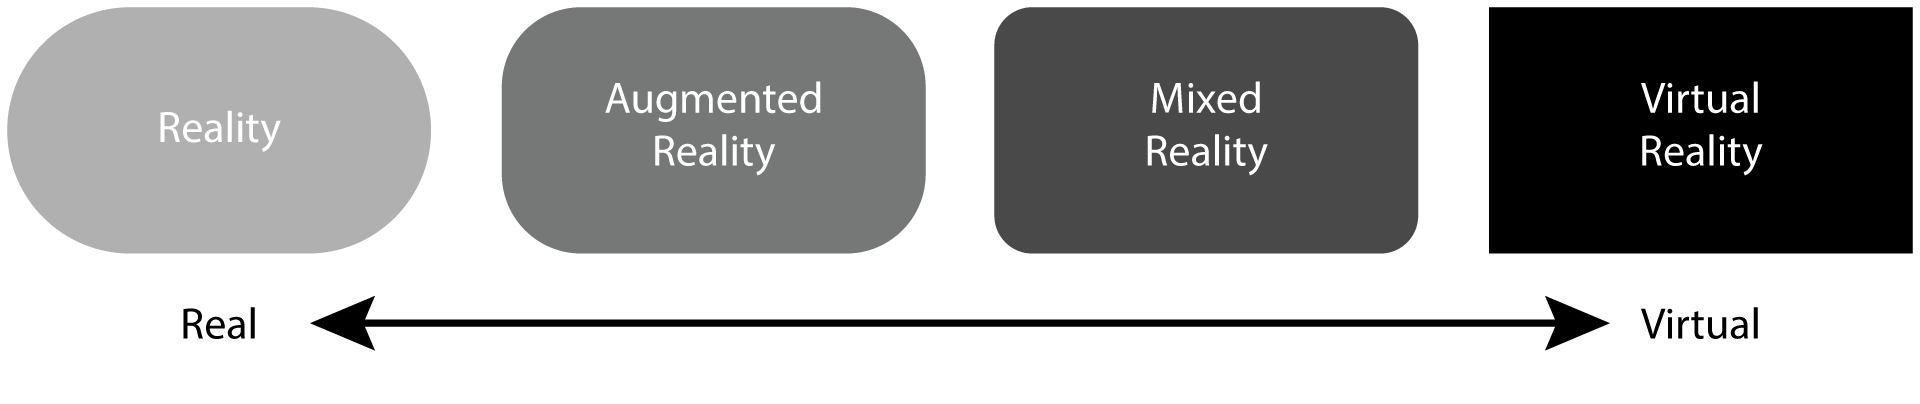
\includegraphics[width=.8\textwidth]{Lifton_continuum_original.png}
	\caption{Lifton's virtual worlds taxonomy.}
	\label{original_lifton_axis.png}
\end{figure}

\begin{figure}[h]
	\centering
	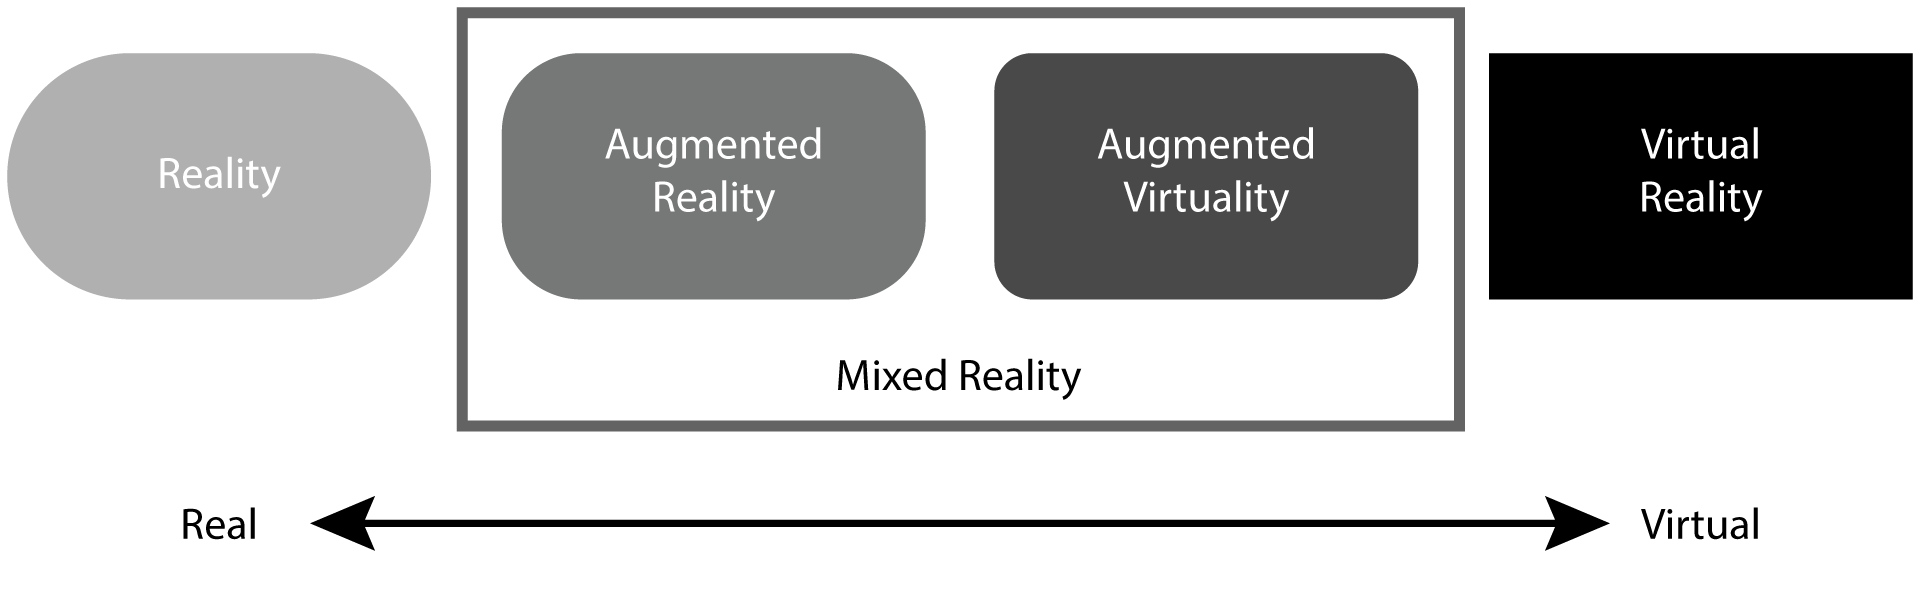
\includegraphics[width=.8\textwidth]{Lifton_continuum_modified.png}
	\caption{Lifton's virtual worlds taxonomy after modification.}
	\label{modified_lifton_axis.png}
\end{figure}

Lifton does however explain that while such a taxonomy can be successfully applied to most alternate realities, with each falling into a different singular category, it does not well address those that feature two complete realities, one real and one virtual, which is one of the distinguishing characteristics of cross reality. He instead presents figure \ref{reality_virtual_reality_sensor_networks.png} to show how sensor/actuator infrastructure causes the real and a virtual environment to merge into a cross reality situation.

\begin{figure}[h]
	\centering
	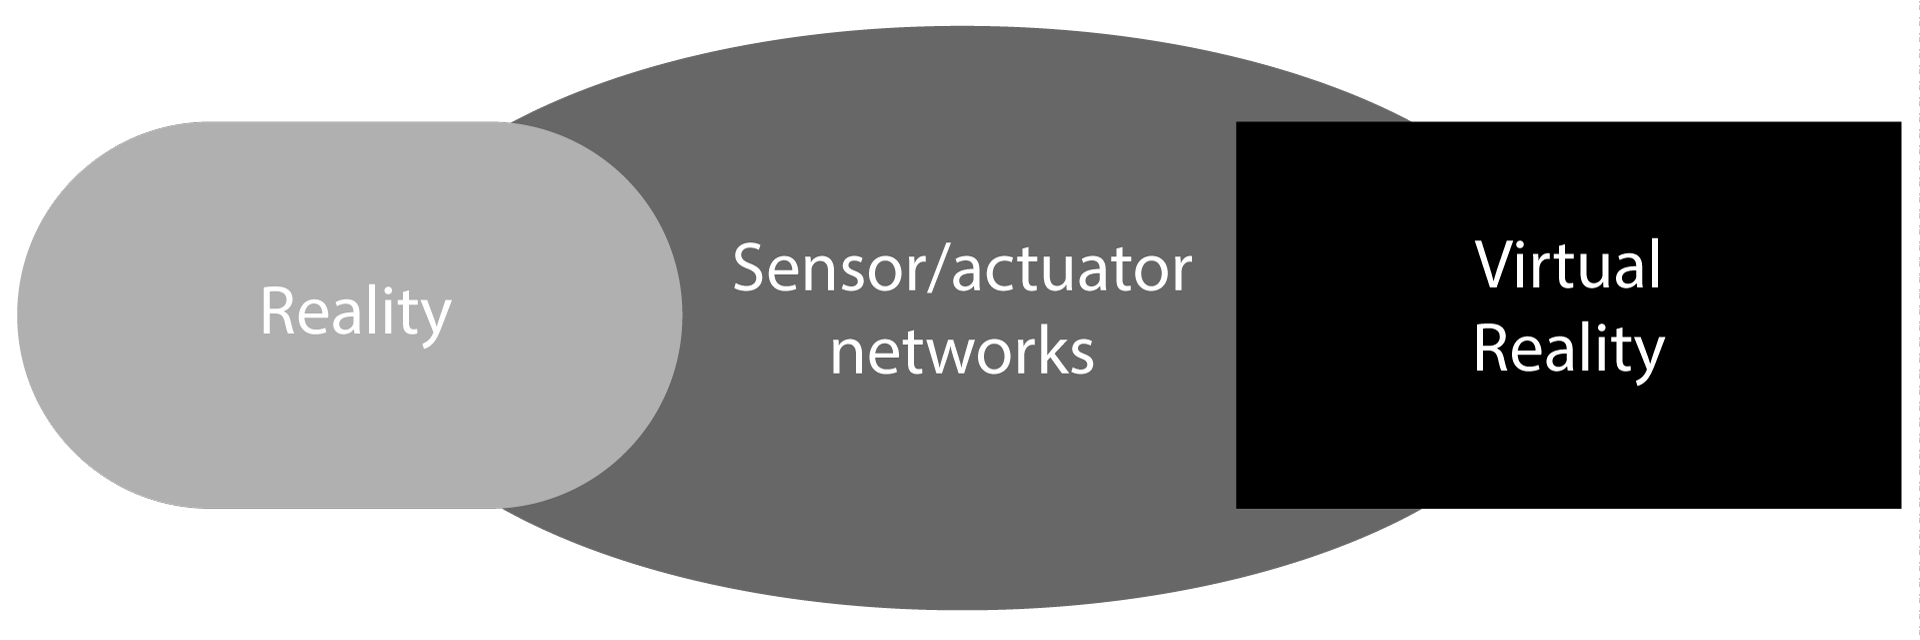
\includegraphics[width=.6\textwidth]{reality_virtual_reality_sensor_networks.png}
	\caption{Sensor/actuator infrastructure merging real and virtual environments into an instance of cross reality.}
	\label{reality_virtual_reality_sensor_networks.png}
\end{figure}

%page 37 of Lifton's thesis

%=========================================================================================================

\subsection{Position of Cross Reality}

\label{positionofcrossreality}

\newcommand{\avxrfootnote}{\footnote{This discussion over the relationship between augmented reality and cross reality also stands for the relationship between augmented virtuality and cross reality, however as augmented virtuality has received less attention in the literature and in commercially available implementations, the discussion uses augmented reality as its example.}}

The position of cross reality in relation to other alternate realities can be visualised using Milgram and Kishino's reality-virtuality continuum. As one of the defining characteristics of cross reality is that it features two environments, both complete unto themselves, the explanation herein distinguishes between environments themselves (depicted in figures \ref{virtuality-continuum-augmented-reality} to \ref{virtuality-continuum-cross-reality-information-flows-dashed.png} by solid ellipses) and where the environmental stimuli that the user is perceiving originate from (depicted by dashed ellipses).

%Ontology - The core meaning within computer science is a model for describing the world that consists of a set of types, properties, and relationship types. There is also generally an expectation that the features of the model in an ontology should closely resemble the real world (related to the object).

Of particular importance is to appreciate the distinction between a cross reality system and an augmented reality system\avxrfootnote{}, as both concepts involve user engagement with both real and virtual content. An augmented reality system features a single environment comprised of the user's real world overlain by and `combined' with~\cite{Billinghurst2014} some virtual content, a \textit{`` `cybrid' environment existing simultaneously in virtual and physical modes''}~\cite{Lichty2014}, with the user perceiving stimuli from this single augmented environment (figure \ref{virtuality-continuum-augmented-reality}). A cross reality system instead features two discrete environments, one real and the other virtual, each complete unto itself (figure \ref{virtuality-continuum-cross-reality-1}), with the user attending either to the stimuli originating from the real environment (figure \ref{virtuality-continuum-cross-reality-2}) or to the stimuli originating from the virtual environment (figure \ref{virtuality-continuum-cross-reality-3}).

\begin{figure}
	\begin{center}
		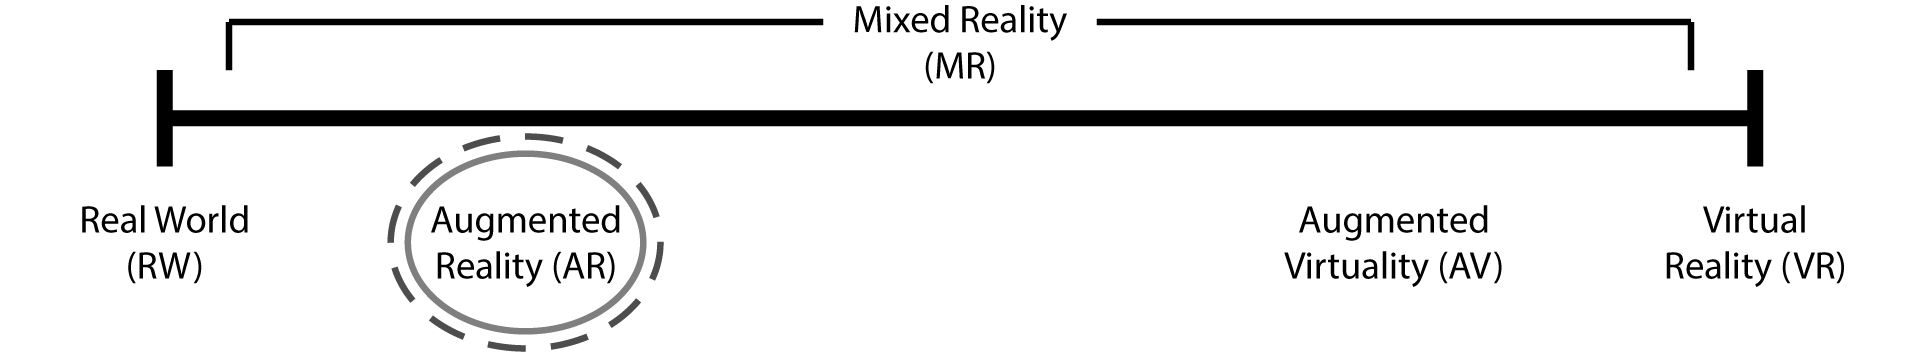
\includegraphics[width=\textwidth]{virtuality-continuum-augmented-reality.png}
		\caption{The single environment of an augmented reality system.}
		\label{virtuality-continuum-augmented-reality}
	\end{center}
\end{figure}

\begin{figure}
	\begin{center}
		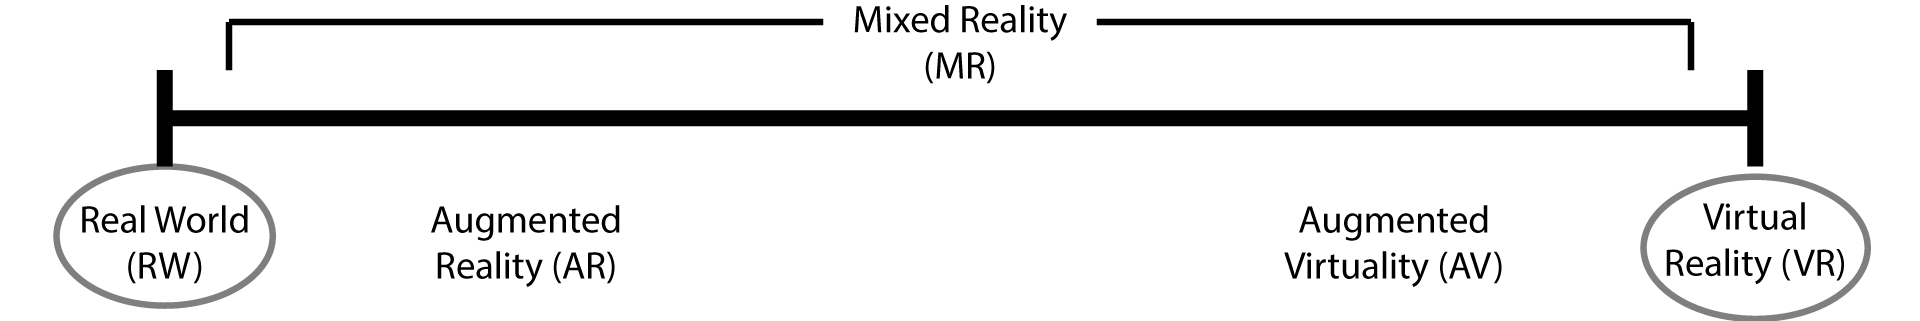
\includegraphics[width=\textwidth]{virtuality-continuum-cross-reality-1.png}
		\caption{The two environments that comprise a cross reality system.}
		\label{virtuality-continuum-cross-reality-1}
	\end{center}
\end{figure}

\begin{figure}[h]
	\begin{center}
		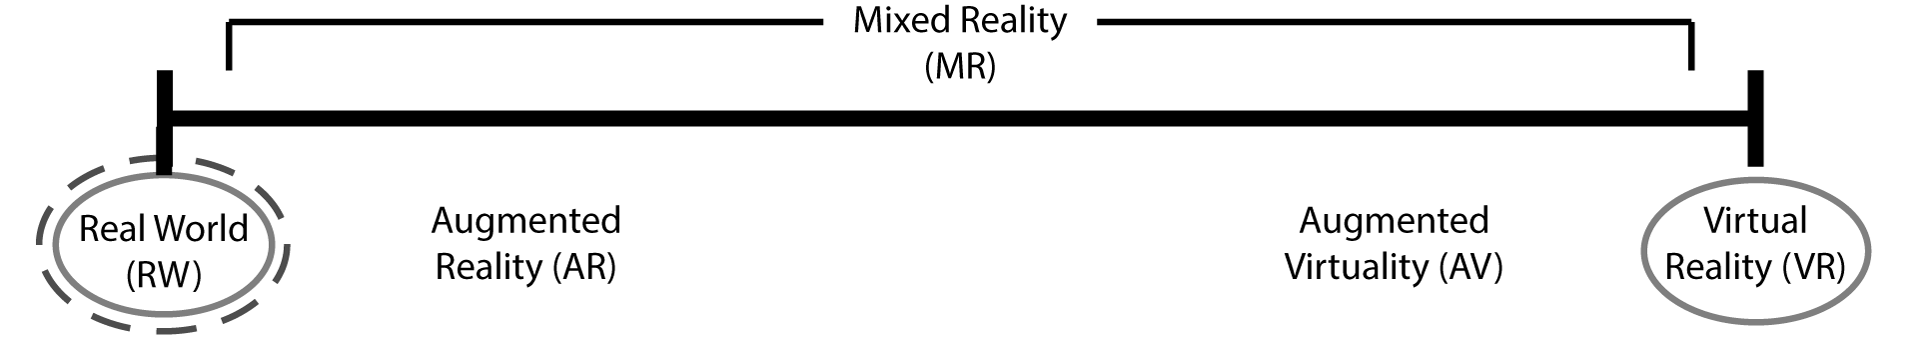
\includegraphics[width=\textwidth]{virtuality-continuum-cross-reality-2.png}
		\caption{A cross reality system with the user attending to real stimuli.}
		\label{virtuality-continuum-cross-reality-2}
	\end{center}
\end{figure}

\begin{figure}
	\begin{center}
		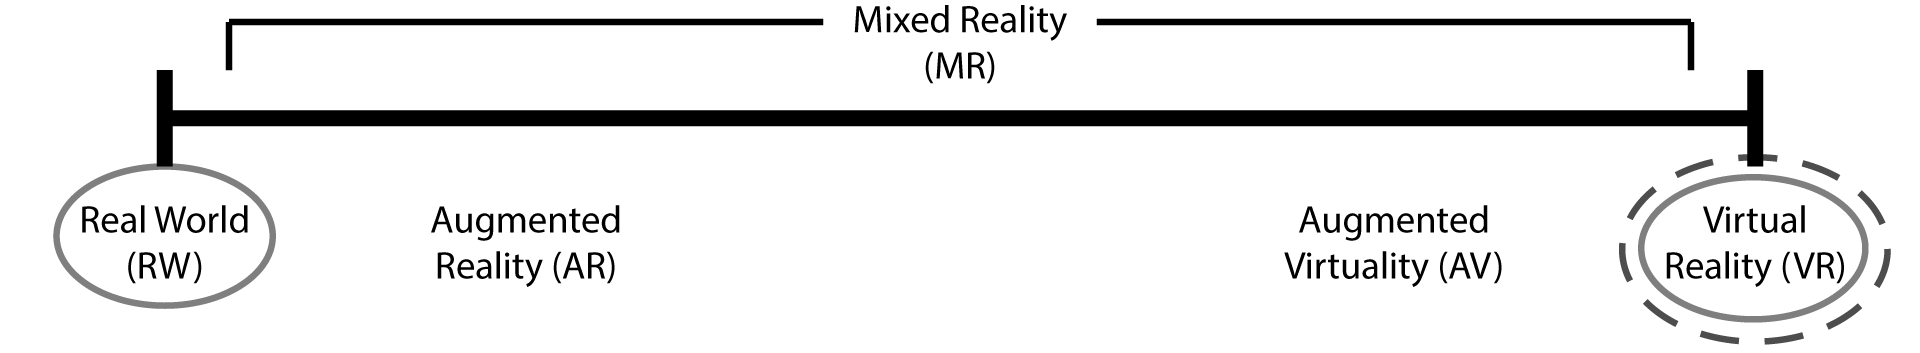
\includegraphics[width=\textwidth]{virtuality-continuum-cross-reality-3.png}
		\caption{A cross reality system with the user attending to virtual stimuli.}
		\label{virtuality-continuum-cross-reality-3}
	\end{center}
\end{figure}

%Similarly to AR, a HR environment likewise constitutes a single physical environment, formed by the seamless introduction of VR content into the real world, rather than two complete environments;

%`physical' quote is HyperReality p158

%HyperReality p26
%\begin{quote}
%	\textit{``\ldots\ virtual people, virtual objects and virtual settings can interact and thereby communicate with real people, real objects and real settings as though they were all part of the same world.''}~\cite{Terashima2001}
%\end{quote}

Although a cross reality system as a whole might be considered a case of mixed reality, whether each of its constituent environments should be considered outwith or within the realm of mixed reality (especially when visualised upon the continuum) is open to debate. Taking the real environment as an example, one could argue that the use of actuators to produce physically observable effects on behalf of controls from the virtual environment constitutes an augmented reality environment. However in adherence with the definition of augmented reality adopted in table \ref{adopted-alternate-reality-definitions} we would not label this an augmented reality environment as we do not have \textit{virtual} objects overlain upon our view of the real environment, but rather \textit{real} physical objects controlled by the actions and events within a discrete virtual environment. So whilst an augmented reality environment falls within the realms of mixed reality, the constituent environments of a cross reality system when considered individually are considered here as occupying the two extremes of the continuum, outwith the mixed reality region and thus their depiction as such in figures \ref{virtuality-continuum-cross-reality-1} to \ref{virtuality-continuum-cross-reality-information-flows-dashed.png}. It is beyond the scope of this chapter to discuss the ontological implications of the `reality' of virtual objects and actions, so the interested reader is referred to Brey~\cite{Brey2014} for further discussion of this subject.

%***this is more to do distribution of the dashed line surrounding the environments, rather than the position of the environments themselves (solid line)***

%However, XR systems that allow simultaneous interaction with both of their constituent environments blur this definition; using a XR platform such as that discussed in this document, a user can transition between perceiving stimuli from each of these environments (figures \ref{virtuality-continuum-cross-reality-2} and \ref{virtuality-continuum-cross-reality-3}) in a manner that allows them to engage with each environment without becoming wholly vacant from the other.

A further distinction between augmented reality and cross reality is made by consideration of Steed's primary environment concept (see discussion in section \ref{milgram&kishino}). For an augmented reality system the primary environment is necessarily real, as augmented reality describes systems in which virtual objects are superimposed upon a view (a background) of a real environment. However for a cross reality system one could argue that the primary environment is either real or virtual, depending upon how the user interacts with the system. For the user that walks through the real environment of a cross reality system and views their unmediated surroundings (including physical actuations triggered by events within the virtual environment), one would intuitively posit that their primary environment is real. But for the user that sits in front of a computer monitor and uses an avatar to walk through the virtual environment of the same cross reality system and hence views the avatar's virtual surroundings (including visualisations of sensor data collected from the real environment), one would posit that their primary environment is virtual. Considering figures \ref{virtuality-continuum-cross-reality-2} and \ref{virtuality-continuum-cross-reality-3} again, one could say that the dashed ellipses thus represent the primary environment for a cross reality system in each of these scenarios respectively.

In relation to the vacancy problem, in scenarios wherein interaction with both real and virtual content is desirable but for which a complete virtual environment is not required, augmented reality circumvents the vacancy problem by virtue of presenting a single mixed reality environment to the user. However for scenarios wherein the use of a complete virtual environment is either beneficial or outright required, the vacancy problem must be mitigated to allow for constructive interaction with these two discrete environments; as is the aim of the cross reality paradigm.

%=========================================================================================================

\section{Parallel Reality}
\label{parallelrealityinbackground}
\newcommand{\PRfootnote}{\footnote{Note that the use of `PR' in the quotation in section \ref{subsec_HyperReality} is a reference to `physical reality' (that author's term for what this thesis simply calls `reality') and is not a reference to parallel reality.}}

The discussion in the previous section highlighted that the first distinguishing feature of cross reality that differentiates it from other alternate realities such as augmented reality and augmented virtuality, is that it features two discrete environments, one real and the other virtual. The second distinguishing feature is the presence of a bidirectional flow of information between these two environments. These features are visualised by figure \ref{virtuality-continuum-cross-reality-information-flows-dashed.png}.

\begin{figure}[h]
	\begin{center}
		
\includegraphics[width=\textwidth]{virtuality-continuum-cross-reality-information-flows-dashed.png}
		\caption{The two environments that comprise a cross reality system, with the bidirectional information flow between them.}
		\label{virtuality-continuum-cross-reality-information-flows-dashed.png}
	\end{center}
\end{figure}

While the parallel reality concept introduced by this thesis also features two discrete environments, one real and the other virtual, that users can freely transition between visually observing, the bidirectional information flow between these environments operates in a different manner. In a cross reality system information flows both ways between the constituent environments and is processed and combined by computational means. In a parallel reality system information still flows in both directions between the environments, but it is processed and combined by the human mind, rather than through computational means. The exception to this observation is the use of sensed real position information in a parallel reality system to maintain the user's vantage point into the virtual environment.

As such, the term \textbf{parallel reality} is proposed to describe this distinct concept, removing the explicit requirement for computationally processed bidirectional information flows in exchange for the implicit human combination of real and virtual information. Parallel reality is thus defined as:

\begin{quote}
	\textbf{Parallel Reality:} A system comprising two environments that the user may freely switch between, one real and the other virtual, both complete unto themselves.
\end{quote}

%Should a bidirectional information flow be introduced to a parallel reality system, or the ability to transition between receiving visual stimuli from either environment be introduced into a cross reality system, one would in effect produce \textit{parallel cross reality}.

Picking up the discussion of primary environments once more, if one follows the reasoning that the primary environment of a cross reality system depends upon the method with which the user interacts with the system, it stands that a parallel reality system can be described as one that provides its user with the ability to change this method and thus change their primary environment at will. In this regard we further distinguish a parallel reality system from an augmented reality system by defining the former as allowing its user to switch between two different primary environments whereas the latter augments one particular primary environment.

%=========================================================================================================

\subsection{Spatial Equivalence in Parallel Reality}

\label{spatial-equivalence}

%(Life on the Screen, p219
\newcommand{\turklevrfootnote}{\footnote{\textit{``For virtual reality to be interesting it has to emulate the real. But you have to be able to do something in the virtual that you couldn't in the real.''}~\cite{Turkle1997}}}

When discussing a parallel reality system that allows its user to transition between two environments, one real and the other virtual, one must consider the relationship between the two environments, namely whether (and if so, to what extent) their layout, dimensions and content relate to each other. We will refer to this consideration as \textit{spatial equivalence}.

This distinction depends partly upon whether one adopts a dualistic concept of virtual space experience, wherein `cyberspace' is a space in its own right with its own logic and metaphysics thus capable of playing host to any number of fantastical things and places, or whether one restricts the virtual environment by following a positivistic understanding of virtual space in which it serves only as a representation of real - using cyberspace for \textit{``creating acceptable substitutes for real \ldots\ environments''} instead of for \textit{``constructing imaginary worlds that are indistinguishable from the real world''}~\cite{Qvortrup2002}. One may also wish to consider this distinction in relation to the different stages identified by Baudrillard between simulacra and simulation, with complete spatial equivalence occupying the first stage, of a faithful image or copy of a profound reality (the positivistic position), zero spatial equivalence occupying the fourth stage, of pure simulation with no relation to anything in reality (the dualistic position), and partial equivalence perhaps occupying the second stage, a perversion of reality, or the third stage, pretending to be a faithful copy of reality~\cite{Baudrillard1994}.

%=========================================================================================================

However one treats virtual space, a parallel reality system would be unrewarding if the real and virtual environments were identical\turklevrfootnote{}. However a virtual environment that shares roughly the same fundamental dimensions and layout as the real environment (representing the same `place') but which presents an \textit{alternative} representation of it has been proven to be a useful modality in previous cross reality research (see section \ref{sec_crossreality}) and it is this arrangement that this thesis explores; in particular where the virtual environment represents the same place as the real environment but at an earlier moment in \textit{time}. This concept of spatially equivalent real and virtual environments has recently been explored under the name `substitutional reality'~\cite{Simeone2015}, but without the ability to switch between the two environments.

One might consider the `Second Earth' concept to be the ultimate realisation of this scenario of spatially equivalent real and virtual environments. The combination of virtual world technology (as in Second Life) with `mirror world' technology (as in Google Earth), Second Earth theorises a virtual simulation/reconstruction of the entire physical world, such that for any location in the real world there is a corresponding location in the virtual world\footnote{\url{http://www.technologyreview.com/Infotech/18911/}}. The parallel reality platforms developed in this thesis focus on individual locations, however it does not take a great leap of the imagination to comprehend the worth of such a system scaled to larger, even global, application.

Although the use cases for parallel reality systems that feature completely unrelated real and virtual environments (including where the virtual environment is entirely fictitious) may seem limited in terms of possible benefits to understanding or knowledge gain when comparing and contrasting the environments, an educated approach to implementing transitions between these environments, that takes similar considerations as the platforms developed in this thesis, does conceivably have purpose. In the opening quote to this chapter, taken from Neal Stephenson's cyberpunk novel \textit{Snow Crash}, the protagonist enquires about the location of another character, both in the real world and in the `Metaverse' - analogous to a virtual world akin to Second Life, accessed via a HMD, comprised of entirely synthetic locations with no counterparts in the real world and which is used to accomplish the same tasks for which today we use the Web. Her response is that \textit{``In  the Metaverse, I'm on a plusbound monorail train. Just passed by Port 35.''} whilst in reality she is at a \textit{``Public terminal across the street from a Reverend Wayne's"}.

There is no spatial equivalence in this scenario between the real environment and the virtual environment; they are not the same `place'. However the protagonist still wishes to be able to experience both by transitioning between them, paying attention to one while travelling through the other. Situations of publicly experienced spatially equivalent and non-equivalent alternate realities are also rife in Vernor Vinge's novel \textit{Rainbows End}:

\begin{quote}
	\textit{``Robert leaned back from the window and reached out to wider universes. Coloured maps appeared before his eyes. These were realities that were geographically far away, not overlaid upon San Diego at all \ldots\ Finally he got a window that promised `public local reality only.' ''}~\cite{Vinge2006}
\end{quote}

While these situations are currently science fiction, recent developments in mobile VR platforms such as Samsung Gear VR\footnote{\url{http://www.samsung.com/global/microsite/gearvr/}} hint that we are not so far away from a time in which members of the general public will wish to multiplex their real environment with a virtual one in this fashion while in public, in the same way that people commonly engage in computer-mediated communication (CMC) via their smartphones at the same time as walking through real environments and conversing with the people around them, creating instances of polysocial reality. If a parallel reality system were to allow interaction between its user and other virtual environment users who are not part of the parallel reality scenario, it is conceivable that polysocial instances would arise with parallel reality users socially engaging both with people in their immediate real environment and with people in their immediate virtual environment, even where the latter are not present in the former. This situation would present \textit{``\ldots\ instances of synchronous polysocial reality, multiple presence \ldots\ being activated in different environments.''}\footnote{Personal correspondence with Sally Applin, polysocial reality author.}

With the majority of players of popular Massively Multiplayer Online games (MMOs) wishing they could spend more time playing, over a fifth even wanting to spend all of their time in game~\cite{Castronova2006}, and with social roles and the community aspect constituting key aspects of these game's popularity~\cite{Castronova2006, Bartle2004}, informing the implementation of transitions between real and virtual in such systems with the findings of the experiments in this thesis into spatially equivalent parallel reality promises to be beneficial to the further development of 3D social CMC in a wider sense.

%=========================================================================================================

\subsection{The Case for Parallel Reality}
\label{caseforpr}
%ARCHEOGUIDE makes the point that AR is good because users are not isolated/completely immersed in a synthetic world - well Mirrorshades allows uers to more fully immerse themselves in a synthetic world, but without becoming isolated in it (eg without becoming ***vacant*** from the real world)

A parallel reality system that presents the user with the choice between immersive visual stimuli from both its constituent environments allows that user to engage with both real and virtual content in a manner that is similar to, but has a number of advantages over, previously explored alternate reality techniques, including augmented reality implementations and cross reality systems:

\begin{itemize}
	\item A parallel reality system is less critical of registration (the accurate positioning/alignment) between real and virtual, as virtual objects are seen as part of a larger virtual environment instead of being rendered atop a view of the real environment~\cite{Azuma1997}.
	\item A parallel reality system can make use of existing virtual reality content without the overhead of decanting/extracting a subset of the virtual components into an augmented reality framework (e.g. manually selecting which objects within the virtual environment are to be displayed over the real environment).
	\item The use of a complete virtual environment allows virtual content to be more encompassing and immersive, allowing total control over lighting, shadows, reflections, particle effects, etc. which would be difficult or impossible for an augmented/diminished reality platform to render atop a view of a real environment.
	\item The vacancy problem is further addressed, but instead of doing so by linking real and virtual environments by sensor and actuator infrastructure as in cross reality, vacancy in both environments is alleviated by furnishing users with the ability to transition between perceiving visual stimuli from them both.
\end{itemize}

Parallel reality platforms are thus well suited to situations in which interaction with the visual stimuli of both real and virtual environments is required and where one or more of the following hold true:

\begin{itemize}
	\item In lieu of accurate registration between real and virtual, there is a strong focus on the virtual environment's atmosphere and immersion~\cite{deamicis:gamebased}.
	\item There is existing virtual reality content.
	\item The visual differences between real and virtual environments are substantial enough that an augmented/diminished reality system would resort to augment or diminish almost the whole real view. While augmented reality \textit{``smears an informational coating over real space''}~\cite{Andersen}, parallel reality presents a complete virtual environment. While augmented reality is beneficial where one wishes the juxtaposition of virtual objects upon what is already present in the real environment, parallel reality is better suited to situations wherein one wishes to present a complete virtual alternative, such as the chapel scenario explored in section \ref{chapel-intro}.
\end{itemize}

%=========================================================================================================

\section{Additional Alternate Reality Definitions}
\label{summaryofadditionalalternaterealitydefinitions}

Table \ref{additional-alternate-reality-definitions} serves as an extension to table \ref{adopted-alternate-reality-definitions} by summarising definitions of the new categories of alternate reality introduced in this section.

\begin{table}[h]
\begin{center}
\begin{tabularx}{\textwidth}{l *{2}{>{\centering\arraybackslash}X}}

\toprule

\textbf{Term} & \textbf{Definition} \\

\midrule

%=========================================================================================================
		
PolySocial Reality (PoSR) & Describes multiple simultaneous social interactions mediated via various CMC technologies.~\cite{Applin2012}. \\

%\hline
\midrule

%=========================================================================================================

Cross Reality (XR) & Systems that feature two environments, one real and the other virtual, both complete unto themselves~\cite{lifton:merging} but enriched by their ability to mutually reflect, influence and merge into one another thanks to bidirectional information flow between them~\cite{kim:practical}. \\

%\hline
\midrule

%=========================================================================================================

Parallel Reality & Systems comprising two environments, one real and the other virtual, each complete unto itself and wherein the user may freely switch between them. \\

%\hline

%=========================================================================================================
\bottomrule
\end{tabularx}
%\end{longtable}
\end{center}
\caption{Additional alternate reality definitions.}
\label{additional-alternate-reality-definitions}
\end{table}

%=========================================================================================================

\section{Alternate Reality Experience}

%\subsection{Presence}
\label{lit-review-presencec}
Any investigation into alternate realities is likely to involve discussion of their experiential aspect and parallel reality should be no exception. The concept of \textit{presence}, the subjective experience of `being in' one place or environment even when one is physically situated in another~\cite{Witmer1998}, features prominently in such discussions. Presence is distinguished from the concept of \textit{immersion}, used here in the context of `immersion as transportation'~\cite{Calleja2014}, which is an objective description of a technology describing the extent to which it is capable of delivering an illusion of reality to the senses of the user~\cite{Slater1997}. In current theoretical models the sense of presence is seen as the outcome, or a direct function of, immersion; the more inclusive, extensive, surrounding and vivd the virtual environment is, and the more similar the transformations in the virtual environment are to those in the real world, the higher the sense of presence~\cite{Constantin2003}.

Also related is the concept of \textit{involvement}, defined in this context as the psychological state experienced as a consequence of focusing one's energy and attention on a coherent set of stimuli and it is theorized that both involvement and immersion are necessary for experiencing a sense of presence~\cite{Witmer1998}.

\subsection{Waterworth and Waterworth's Three Dimensions of Virtual Experience}
\label{waterworthandwaterworth}
\newcommand{\presencefootnote}{\footnote{\textbf{Presence} in the context of this model is defined as a state of heightened perceptual processing of environmental stimuli (\textit{``a psychological focus on direct perceptual processing''}~\cite{Waterworth2001}) accompanied by lessened conceptual reasoning, covering cases both in which the environmental stimuli originate from the subject's immediate real surroundings (\textit{unmediated presence}) and when the environmental stimuli originate from a remote real environment, virtual environment or mixed reality environment (\textit{mediated presence})~\cite{Mantovani2010}.}}

\newcommand{\absencefootnote}{\footnote{\textbf{Absence} is defined as \textit{``a psychological focus on \ldots\ conceptual processing''}~\cite{Waterworth2001}, as \textit{``presence in an exclusively mental activity''}~\cite{Giuseppe2014}, with total presence (in the above definition) and total absence representing opposite poles along the continuum of the focus of attention axis~\cite{Mantovani2010}.}}

Waterworth and Waterworth present the \textit{three dimensions of virtual experience} model (reproduced in figure \ref{focus-locus-sensus-original} from the original in~\cite{Waterworth2001}) for visualising and discussing virtual/physical experience in terms of three separate `axes of attention', one of which relates closely to the popular use of the term presence in the wider alternate reality literature. This division of the concept of virtual/physical experience, which allows the separate consideration of which environment a user is attending to the stimuli of and how \textit{much} they are attending to these stimuli (wherever they may come from), is diagnostic in the investigation of the experience of parallel reality systems that promote transition between the stimuli of two discrete environments, particularly where the concept of the `break in presence' is concerned (see section \ref{background-breaks-in-presence}).

\begin{figure}[h]
	\begin{center}
		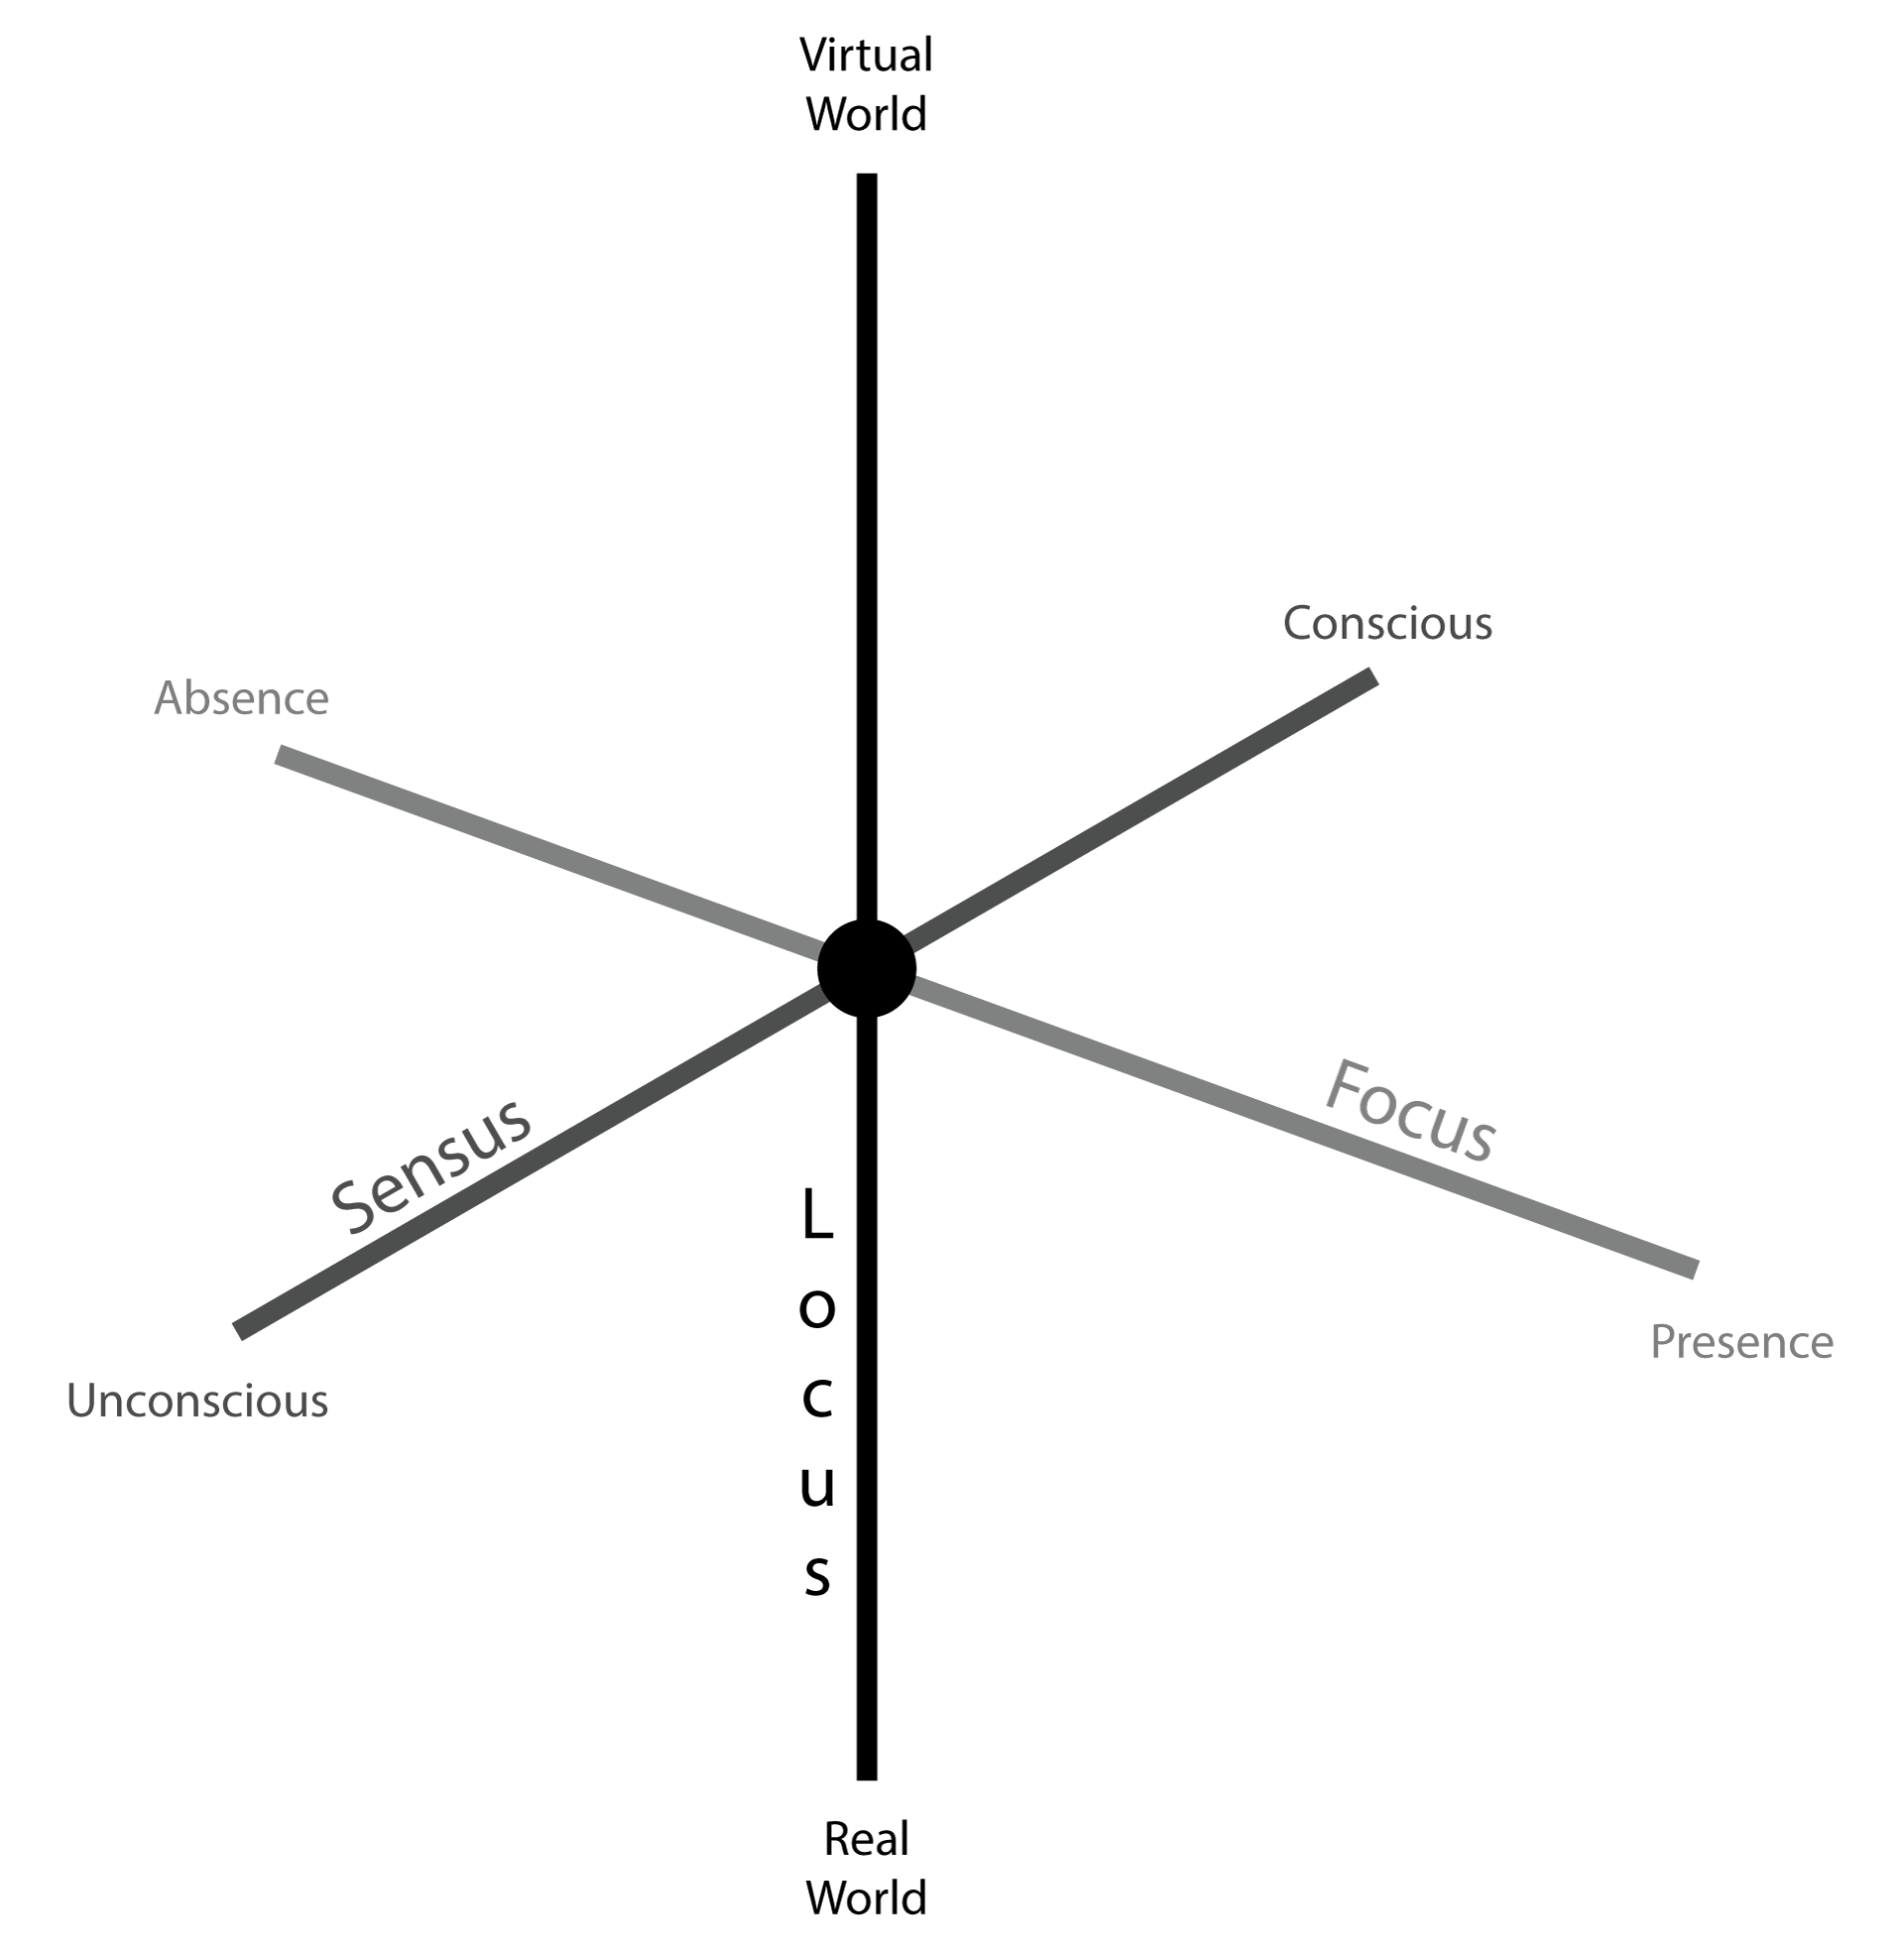
\includegraphics[width=.6\textwidth]{focus-locus-sensus-original.png}
		\caption{The three dimensions of virtual experience model.}
		\label{focus-locus-sensus-original}
	\end{center}	
\end{figure}

In the three dimensions of virtual experience model:
\begin{itemize}
	\item The \textit{locus of attention} axis represents the environment where the stimuli that the user is perceiving originate from.
	\item The \textit{focus of attention} axis represents the balance between conceptual/abstract reasoning and perceptual/concrete processing, where complex conceptual reasoning (or `distraction' from percepts~\cite{Chalmers2014}) results in little attention being paid to processing environmental percepts (whether originating from real stimuli, virtual stimuli, or a mix) thus reducing presence\presencefootnote{} in that environment toward its antithesis $-$ absence\absencefootnote{}.
	\item The \textit{sensus of attention} axis represents the level of conscious arousal (or `wakefulness'~\cite{Laureys2009}) of the user, whether directed toward percepts originating from real stimuli, virtual stimuli, a mix of both, or not directed toward any percepts in the case of completely `absent' conceptual reasoning, a concept clarified by the authors:

\begin{quote}
	\textit{``Presence arises from active awareness of our embodiment in a present world around us. Presence is not consciousness, and we may be highly conscious while feeling absent, at those times when we are relatively unaware of our own embodiment.''}~\cite{Waterworth2014}
\end{quote}
\end{itemize}

In this model, the notion of involvement relates closely to the focus of attention axis; heightened involvement pertains to concentrating on environmental stimuli or meaningfully related activities and events, while heightened focus pertains to increased perceptual/concrete processing; lessened involvement pertains to a preoccupation with personal problems or activities occurring outwith the environment of interest, while lessened focus pertains to increased conceptual/abstract reasoning.

%=========================================================================================================

\subsection{The Combined Milgram/Waterworth Model}
\label{combined-milgram-waterworth-model}
With the locus of attention axis representing the environment from which the stimuli the user is perceiving originate from, a relationship can be drawn between the Waterworth model and Milgram and Kishino's reality-virtuality continuum, with the latter considered here to be analogous to the locus of attention axis. The combination of these two models in this manner gives rise to the combined Milgram/Waterworth model which is shown by figure \ref{focus-locus-sensus-with-virtuality-continuum} and allows for a novel method of visualising the experience of using alternate reality systems, including those that implement parallel reality.

\begin{figure}[h]
	\begin{center}
		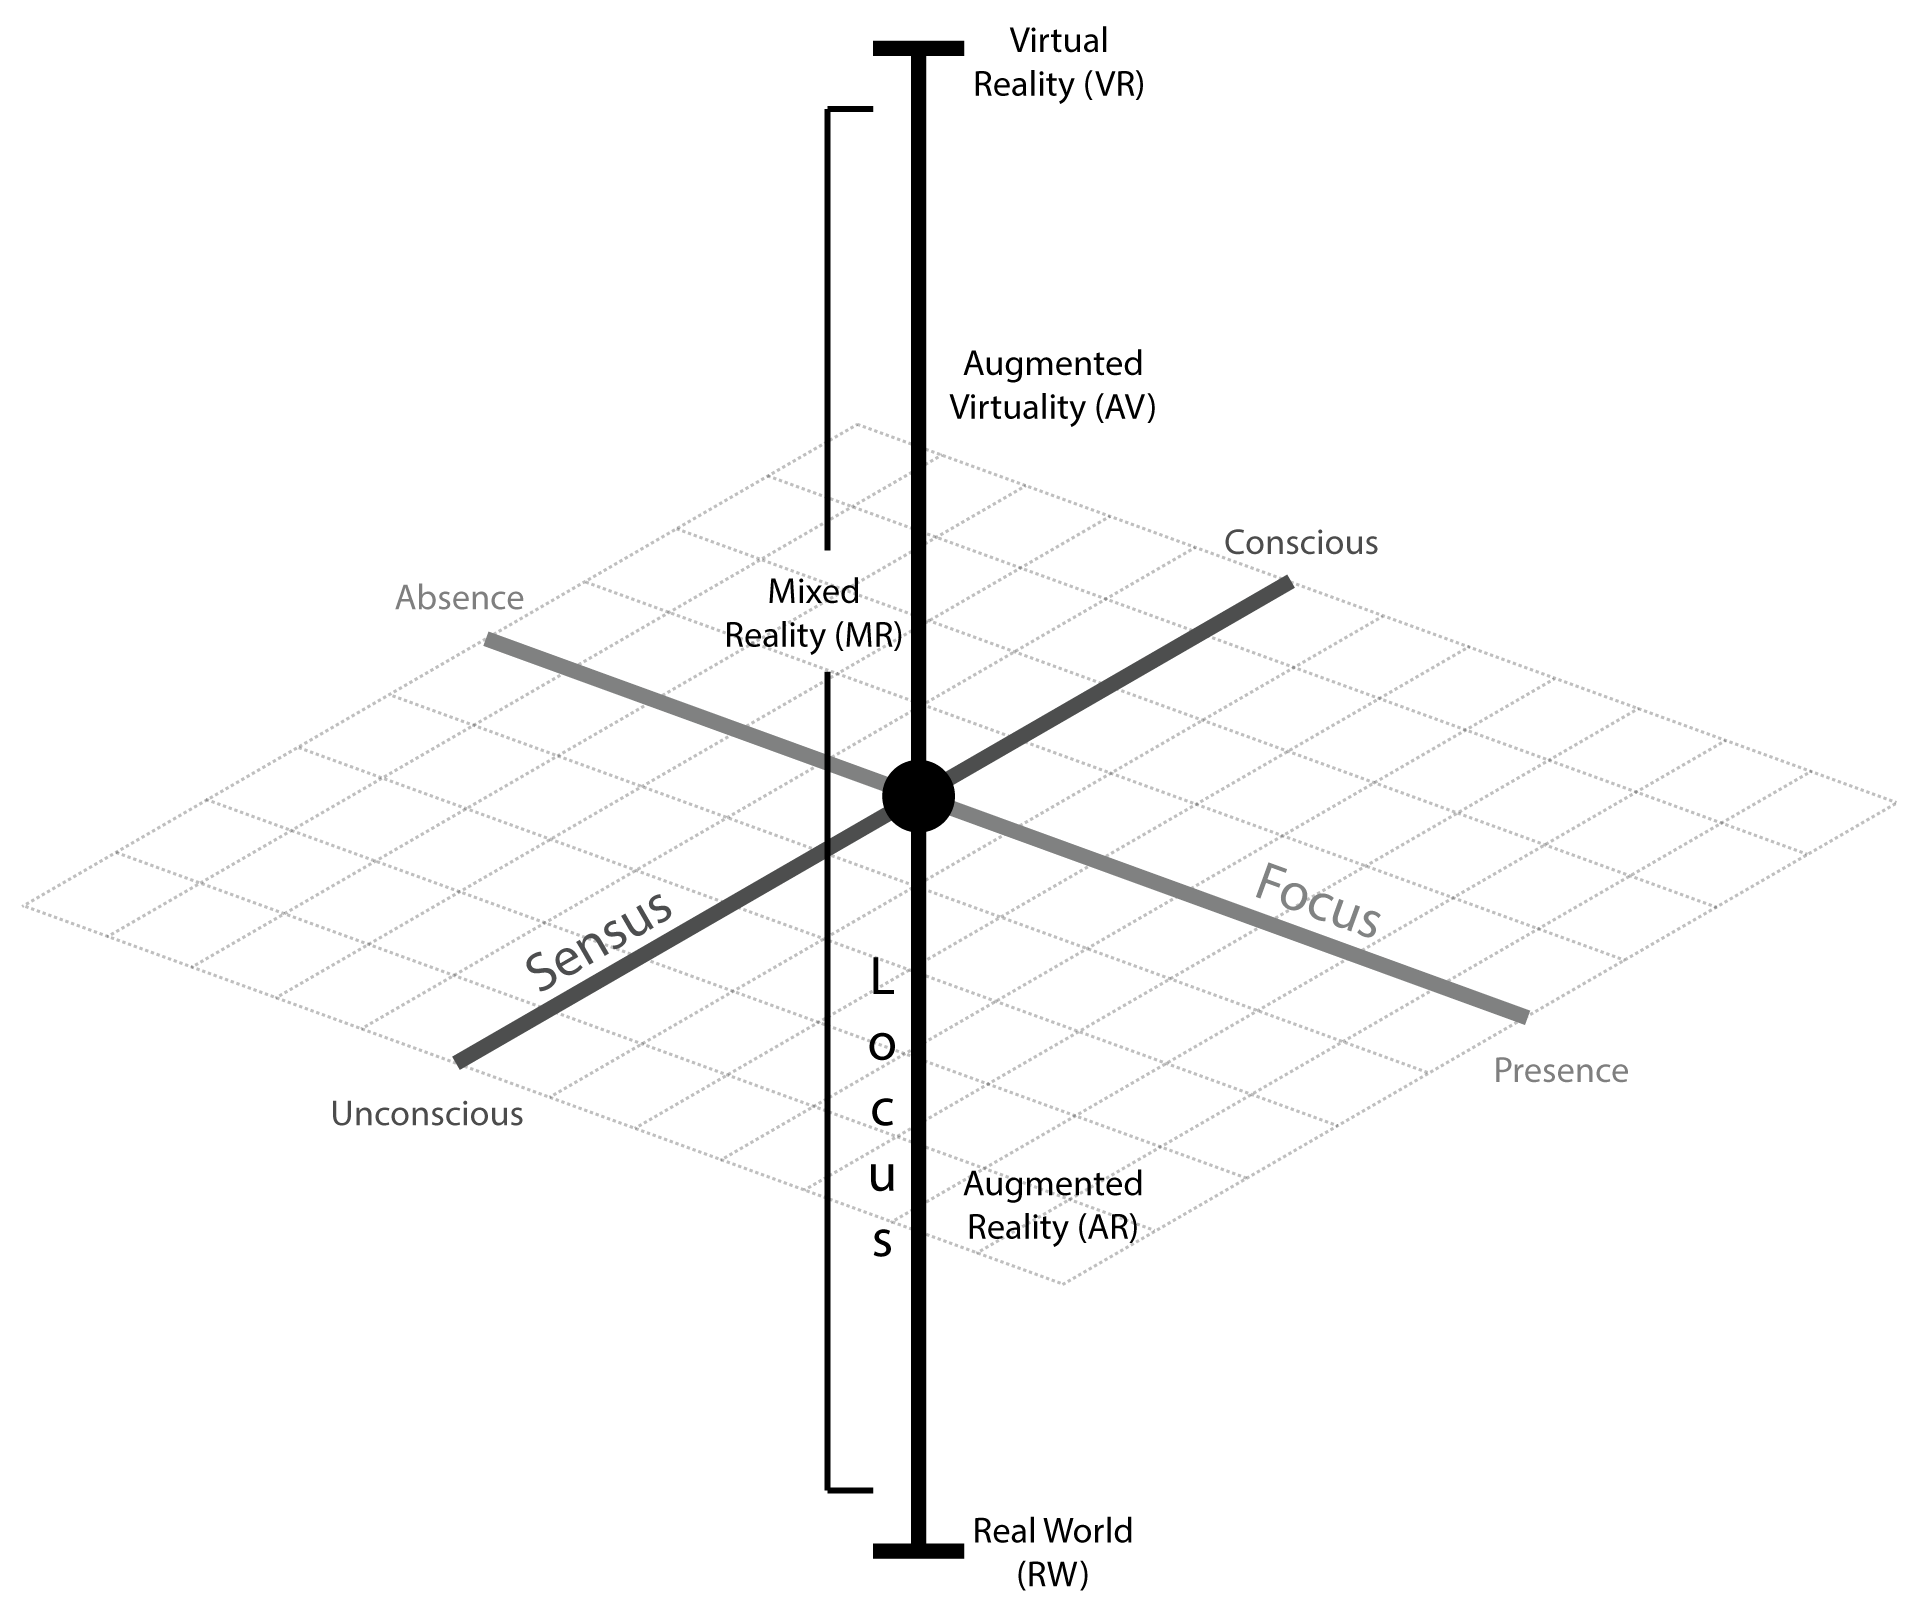
\includegraphics[width=.8\textwidth]{focus-locus-sensus-with-virtuality-continuum-updated-with-grid.png}
		\caption{The combined Milgram/Waterworth model.}
		\label{focus-locus-sensus-with-virtuality-continuum}
	\end{center}	
\end{figure}

Studying the combined Milgram/Waterworth model shows more clearly that the balance between presence and absence can relate to any environment upon the locus of attention axis, as confirmed by Waterworth and Waterworth:

\begin{quote}
	\textit{``We may feel hardly present at all in the physical world (a state we call absence) if nothing is happening there that is of interest or that impacts on our well-being, and so it is with mediated presence.''}~\cite{Waterworth2014}
\end{quote}

Furthermore one can postulate as to the essence of Lifton's vacancy with regard to the combined Milgram/Waterworth model (and thus to the experience of presence in general). Lifton's original definition presents vacancy as the `absence' of a person from one world while they are participating in the other, however the use of this term in Lifton's context differs to its use in the combined Milgram/Waterworth model. Lifton's absence refers to the inability to simultaneously perceive environmental stimuli from \textit{``more than one place (reality)''} while the absence of the combined Milgram/Waterworth model refers to increased conceptual/abstract reasoning resulting in a reduction of perceptual/concrete processing of all environmental stimuli. In terms of the combined Milgram/Waterworth model, the vacancy problem should be thought of as referring to the largely singular nature of a user's position upon the locus of attention axis.

%and the ability of a parallel reality platform toward reducing the problem, by allowing a user to `participate' in two environments at once, can be visualised either as extending the occupiable position upon the locus of attention axis from a singular position to a pair of positions (or as a range between two positions), or as reducing the deflection experienced upon the focus of attention axis from presence toward absence when performing a transition between two positions upon the locus of attention axis.

%The Sensus Dimension - the importance of being awake in class
%"Even as we sleep dreamlessly..." (example of being 'unconscious' in this regard)

%fourth axis is alterity, between hermeneutics and embodiment

%=========================================================================================================

\subsection{Experience in Parallel Reality}

\label{transitions_in_parallel_reality}

In terms of the combined Milgram/Waterworth model, the novel aspect of parallel reality can be visualised as the ability it imparts upon its user to freely switch their locus of attention between equivalent vantage points in real and virtual environments. In order to achieve the highest quality of experience with this style of interaction it is vital to determine how best to implement these transitions; that is, to mitigate the increased cognitive load (manifesting as increased conceptual reasoning and reduced perceptual processing) required to comprehend each transition, as this will detract from engagement with the environments and reduce the user's willingness to perform subsequent transitions.

%In the systems developed by this thesis the users maintain mobility, such that they can move around the two environments in tandem, thus extending existing XR platforms that featured static locations at which a user in the real environment could see into the virtual and vice-versa. This combination of unhindered mobility with the ability to transition between real and virtual stimuli thus alleviates the vacancy problem.

%This is achieved by the user performing transitions between RW visual stimuli and VR visual stimuli, both presented via their HMD. This extends existing XR research by allowing the user to engage with the visual stimuli of the VR component of a XR system from any position and at any time.

Some researchers support the notion that in systems where more than one environment competes for the user's locus of attention there is an `all or nothing' Gestalt switch between awareness of one environment and the other~\cite{Slater2002}. Considering a parallel reality system, this notion would expect a substantial increase in cognitive load upon each transition between real and virtual environments. However the position adopted by this thesis is of the contrary opinion; that switching locus of attention from the stimuli of one environment to those of another does not completely overrule the user's awareness of the former. Instead, both environments can be perceived at the same time (albeit one to a lesser extent)~\cite{Ijsselsteijn2001} and when engaging with virtual content a user's focus can even be said to typically be \textit{shared} between the real and the virtual environments~\cite{Waterworth2001}, leading to a notion of `distributed' presence, or simultaneously experiencing a sense of presence in multiple environments.

This latter position is particularly apt for situations wherein the real and virtual environments share the same fundamental layout and dimensions (spatial equivalence, see section \ref{spatial-equivalence}), as those of the parallel reality systems explored within this thesis do, as inherent familiarity between two environments intuitively reduces the cognitive load associated with transitioning between them.

Furthermore, the notion of experience of presence as changing continually from moment-to-moment~\cite{Heeter2003, Ijsselsteijn1998} lends confidence to the successful mitigation of the increased cognitive load associated with these transitions to manageable levels. One might even liken this `switching' between real and virtual to the `cycling through' behaviour observed in users of virtual communities, which stemmed from the `window' concept of modern computer operating systems~\cite{Turkle2004} and accelerated with mobile devices to the point where for many users today rapid cycling stabilizes them into a sense of `continual copresence', where even just a mobile phone brings them into a world of continual partial attention to any particular subject or environment~\cite{Turkle2011}. The advent of mobile phones has previously been credited with allowing a person to \textit{``be in many places at once''} and to play multiple roles~\cite{Terashima2001}. The term polysocial reality was introduced to describe situations like this, of multiplexing physical reality with Web-based social networks and apps for Internet mediated social interaction~\cite{Applin2012}. As it has been shown that \textit{``effective interaction among participants is a contributing factor to presence''}~\cite{Terashima2001}, the importance of social interaction upon presence should not be understated.

%HyperReality p148

%=========================================================================================================

\subsection{Breaks in Presence}

\label{background-breaks-in-presence}

No matter how smooth the transition between real and virtual, the process is expected to nonetheless result in some heightened cognitive load, a temporary `break in presence' (BIP), as the user comes to terms with the new environment presented to them and comprehends its relation to the other environment that they were just perceiving. The definition of break in presence adopted herein is that introduced by Waterworth and Waterworth for the purposes of their three dimensions of virtual experience model~\cite{Waterworth2001}. Here, a break in presence represents a movement along the focus of attention axis away from presence in either a real, a virtual, or a mixed reality environment and toward absence. This differs to Slater and Steed's earlier usage of the term~\cite{Slater2000} wherein they considered presence in terms of `virtual presence', where a break in presence is a Gestalt switch from a sense of presence in a virtual environment to a sense of presence in the real environment.

\begin{quote}
	\textit{``When in a virtual environment, presence is typically shared between the VR and the physical world. `Breaks in presence' are actually shifts of presence away from the VR and toward the external environment. But we can also have `breaks in presence' when attention moves toward absence - when an observer is not attending to stimuli present in the virtual environment, nor to stimuli present in the surrounding physical environment''}~\cite{Waterworth2001}
\end{quote}

The Waterworth model considers presence in terms of attending to stimuli from either a real environment, a virtual environment, a mixed reality environment, or even multiple environments, with a break in presence representing absence in the sense of heightened conceptual load and the resultant reduced perceptual processing of environmental stimuli, no matter the provenance of those stimuli. This usage better fits the situations invoked by the parallel reality concept, which is concerned with intentionally and willingly switching engagement between stimuli from both real and virtual environments, rather than engaging with stimuli from only a virtual environment in a scenario wherein stimuli from the real environment are considered a `distraction'.

This difference between the Steed and Waterworth uses of break in presence can be visualised by considering the axes of the combined Milgram/Waterworth model. In the Steed definition a break in presence represents a movement upon the locus of attention axis from the virtual world to the real world. In the Waterworth definition a break in presence represents a movement upon the focus of attention axis from presence to absence, regardless of position upon the locus of attention axis.

%=========================================================================================================

\subsection{Visualising Transitions and the Extended Vacancy Problem}

Visualised using the combined Milgram/Waterworth model, the transitions of a parallel reality system are an oscillation between two different positions upon the locus of attention axis. Figure \ref{focus-locus-sensus-with-virtuality-continuum-with-transition} shows an example where a user performs a smooth transition between perceiving stimuli from a fully real environment and a fully virtual environment.

\begin{figure}[h]
	\begin{center}
		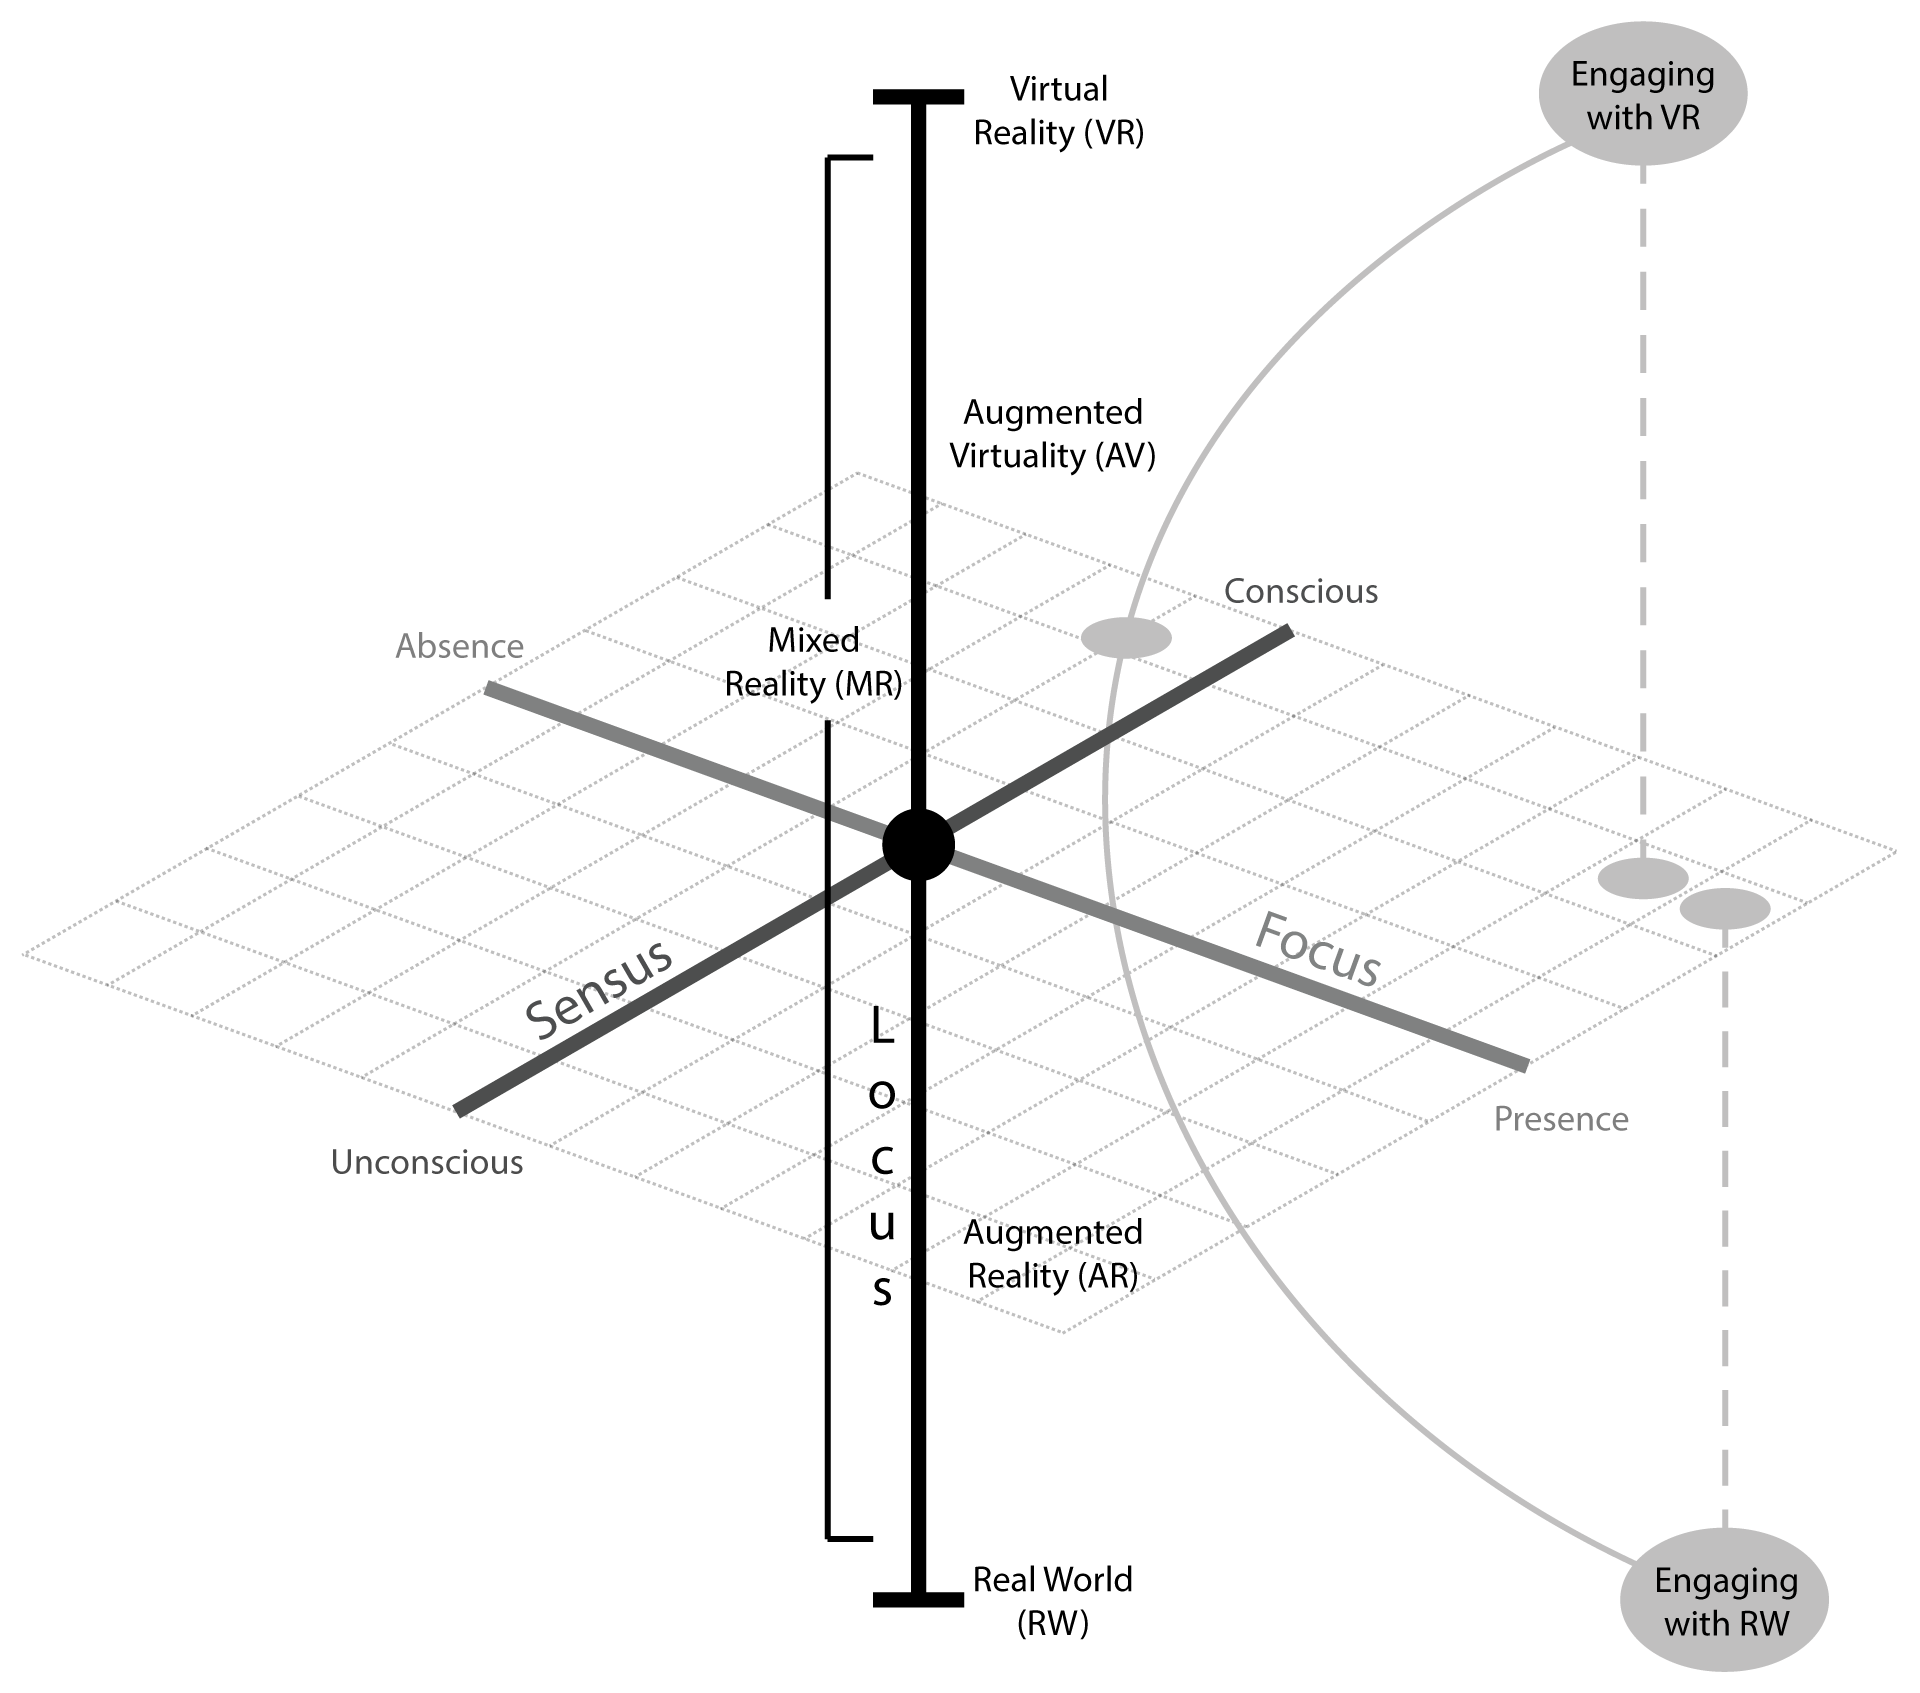
\includegraphics[width=.8\textwidth]{transition-rw-vr.png}
		\caption{Visualisation using the combined Milgram/Waterworth model of the theorised experience of a user of a HMD based parallel reality system performing a smooth transition between its constituent real and virtual environments.}
		\label{focus-locus-sensus-with-virtuality-continuum-with-transition}
	\end{center}	
\end{figure}

Heightened cognitive load required to comprehend the transition is represented by a temporary movement upon the focus of attention axis from presence toward absence (a break in presence). With the ability of a wide field of view (FOV), stereoscopic 3D, head-tracked HMD (such as that used by the Mirrorshades platform developed in this thesis) to produce immersive virtual reality visual stimuli that require fairly limited cognitive processing and our inherent ability to engage with our real surroundings without significant cognitive load, focus is represented as being high (toward the presence extreme) when attending to stimuli from either the real or virtual environments.

Sensus is expected to be largely task dependent, however when performing a task that involves actively engaging with the visual stimuli from either/both of the real and virtual environments it is expected to be high (toward the conscious extreme). Upon triggering a transition, sensus is expected to increase, as the user centres their attention upon relating the visual stimuli from the new environment to those they were just perceiving from the other environment.

Transitions between the virtual world and the real world can be implemented in multiple different manners and it is expected that users may prefer different implementations in different situations, surroundings and scenarios. Preference toward a particular implementation is posited to correlate with a less severe break in presence being experienced upon its execution, indicating a greater reduction in the magnitude of the deflection experienced upon the focus of attention axis from presence toward absence when performing the transition.

With Lifton's vacancy being visualised upon the combined model as the largely singular nature of a user's position upon the locus of attention axis (section \ref{combined-milgram-waterworth-model}) and the parallel reality concept hoping to allow users to more freely oscillate between two positions upon the locus of attention axis, success in mitigating deflections upon the focus of attention axis when performing transitions, allowing multiple positions upon the locus of attention axis to be occupied, can be related to success in mitigating vacancy. This observation leads to an extended definition of the vacancy problem:

\begin{quote}
	\textbf{The Extended Vacancy Problem} - Performing a transition between two environments upon the locus of attention axis of the combined Milgram/Waterworth model is accompanied by a deflection upon the focus of attention axis from presence towards absence.
\end{quote}

By investigating several different transition implementations, identifying and quantifying preferences toward them in different situational states, this thesis explores the relationships between transitions and the successful mitigation of the extended vacancy problem.

%=========================================================================================================

%\subsection{Parallel Reality and the Combined Milgram/Waterworth Model}





%Whilst continued exposure to the platform is expected to reduce the severity of the BIPs, mitigating their severity from the outset (reducing the displacement from the presence extremum downwards toward absence) through informed execution of the transitions between RW and VR is believed to be important to the overall quality of experience that users receive.

%absent-mindedness - caused by increased attention toward a single object of focus (hyperfocus, eg the object of focus is the switch)
% or caused by distraction (again, the switch)



%=========================================================================================================
%=========================================================================================================


%=========================================================================================================
%=========================================================================================================
%=========================================================================================================
%=========================================================================================================
%=========================================================================================================
%=========================================================================================================
%=========================================================================================================
%=========================================================================================================
%=========================================================================================================
%=========================================================================================================


%Users are free to explore and interact with either environment in relative isolation from the other, even if their interactions in one trigger changes in the other, however simultaneous interaction and exploration with both environments has largely remained without systematic investigation.

%This is largely because users exploring and interacting with the real environment do not have a convenient manner of also exploring and directly interacting with the virtual environment, as such interaction usually relies upon the use of software run on a desktop or laptop computer which is not conducive to mobile use. Using a laptop computer whilst walking around is far from convenient and using a desktop computer obviously limits the user's interaction with the real environment to that immediately around the location of the  computer and results in a disjoint relationship between their physical position in the real environment and the location of their avatar in the virtual environment when they navigate their avatar away from the respective position of their computer. This situation has been called `the vacancy problem'; an apparent vacancy from one environment whilst engrossed in the other.




%=========================================================================================================
%=========================================================================================================





%=========================================================================================================

%Marie Kim et al at The Electronics and Telecommunications Research Institute, Korea, explain the cross reality paradigm well in terms of its principle features

%\begin{quote}
%\textit{``The important point of X-reality is a paradigm shift from single-directional information flows to bidirectional information flows between two worlds.''}
%\end{quote}

%and also how it can be employed for simultaneous presence in real and virtual environments

%\begin{quote}
%\textit{``The differential characteristic of X-reality is that it can augment user's engagement in the experiences of virtual presence and virtual world. Ultimately, it results in the human life span extension from the only real world to both worlds.''}
%\end{quote}





%Paradiso in IEEE Pervasive, Cross Reality Environments ~\cite{Paradiso2009} \textbf{***check this is the right citation***}

%\begin{quote}
%\textit{We call the ubiquitous mixed reality environment that comes from the fusion of these two technologies cross-reality. Sensor networks can tunnel dense real-world information into virtual worlds, where this data is interpreted and displayed to dispersed users. Interaction of virtual participants can incarnate into the physical world through a plenitude of diverse displays and actuators. We can envision a user's interface into this environment as an extension of human perception and interaction, augmenting our five senses well beyond the canonical ``here and now'' and redefining the meaning of presence.''}
%\end{quote}



%\begin{quote}
%\textit{``We see cross-reality precipitating when diverse and ubiquitous sensor and actuator networks meet pervasively shared online virtual worlds, where phenomena freely tunnel between real and contrived continua at a multitude of ``wormholes'' opened by densely deployed networked devices, seamlessly adapting the level of immersion to match a variable ecology of available interfaces and user context or preference.''}~\cite{Lifton2009}
%\end{quote}


%=========================================================================================================

\section{Summary}
Decades of research into alternate realities has furnished us with a rich continuum of approaches and technologies for creating, combining, augmenting and diminishing real and virtual environments. Many of the alternate reality labels that are now becoming commonplace are concerned with presenting a different environment to the user's real surroundings (as in telepresence and virtual reality) or mixing additional information into the user's view of their real or virtual surroundings (as in augmented reality and augmented virtuality).

Although less thoroughly investigated, the concept of creating an alternate reality system by combining two complete environments, one real and the other virtual, into a cross reality system presents an interesting avenue for furthering alternate reality techniques and applications, in particular to addressing the vacancy problem that affects users when trying to distribute their attention between two environments. Previous cross reality research has focussed upon alleviating this vacancy problem by integrating sensor and actuator infrastructure into the constituent real and virtual environments of a system, such that actions and events in one environment could manifest into the other. However direct visual engagement with both environments was not often possible in these systems and only from predetermined, static locations.

Parallel reality has been introduced as a new category of alternate reality that allows its user to visually engage with both a real and a virtual environment at any position, freely switching between them at any time. In trading the sensor/actuator infrastructure of a cross reality system for direct visual engagement with both environments, the parallel reality concept further addresses the vacancy problem by truly providing \textit{``the means to be in more than one place (reality) at a time''}\cite{Lifton2007a}.

The combined Milgram/Waterworth model has been introduced as a method for visualising alternate reality experience, including those of parallel reality systems, and in relation to this model the definition of the vacancy problem has been extended to allow for the success of parallel reality systems at mitigating vacancy to be explored.